\documentclass[a4paper,fleqn]{cas-sc}

\usepackage{amsmath,amssymb,bm}
\usepackage[numbers]{natbib}
\usepackage{booktabs,multirow}
\usepackage[ruled,linesnumbered]{algorithm2e}
\usepackage{graphicx}
\usepackage{xcolor}
\usepackage{url}
\usepackage{enumitem}
\usepackage{placeins}
% cas-sc loads hyperref; configure it without reloading the package.
\hypersetup{colorlinks=true,citecolor=blue,urlcolor=blue,linkcolor=blue}
\graphicspath{{figures/}}
\setlength{\emergencystretch}{2em}

% The CAS class prints an ORCID footnote even when no ORCID is supplied.
% Preserve the standard output when metadata is present and suppress only the empty note.
\ExplSyntaxOn
\RenewDocumentCommand \printorcid { }
  {
    \seq_if_empty:NF \g_stm_orcid_seq
      {
        \group_begin:
        \tex_let:D \thefootnote \relax \footnotetext
          {
            \raggedright
            \textsc{orcid}(s):\c_space_token
            \seq_use:Nn \g_stm_orcid_seq { ;~ }
          }
        \group_end:
      }
  }
\ExplSyntaxOff

\bibliographystyle{elsarticle-num}

\newcommand{\client}{\mathcal{K}}
\newcommand{\dataset}{\mathcal{D}}
\newcommand{\loss}{\mathcal{L}}
\newcommand{\graph}{\mathcal{G}}
\newcommand{\rules}{\mathcal{R}}
\newcommand{\jsd}{\mathrm{JSD}}
\newcommand{\KL}{\mathrm{KL}}

\begin{document}

\let\WriteBookmarks\relax
\def\floatpagepagefraction{1}
\def\textpagefraction{.001}
\shorttitle{FLEN: Conflict-Aware Federated Legal Language Modeling}
\shortauthors{Robert J.}

\title[mode = title]{FLEN: A Conflict-Aware Federated Framework for Cross-Jurisdiction Legal Language Modeling}

\author[1]{Robert J.}
\affiliation[1]{organization={Independent Research Project}}

\begin{abstract}
Recent advances in legal large language models and federated adaptation support collaborative legal information processing while keeping institutional case records local.

However, existing pipelines often interpret predictive disagreement as legal conflict without considering differences in applicable authority. They also provide limited control over local adaptation that can degrade model performance. Moreover, they often lack a coordinated process for verifying generated arguments before reaching a final judgement.

To address these limitations, we propose the Federated Legal Expertise Network (FLEN). First, FLEN checks whether client outputs are comparable under the target authority and weights compatible contributions according to their conflict exposure. Second, it separates shared and private adaptation into independent LoRA branches and uses held-out local records to select private updates. Third, distinct agents develop and challenge legal arguments, verify the supporting evidence, and synthesize a final judgement.

Experiments on CaseHOLD compare FLEN components with FedAvg, FedProx, FedAdam, and Ditto under matched protocols. Across five seeds, gating improves test accuracy over unguarded personalization by 2.50 and 2.64 percentage points at two fixed training budgets. MultiEURLEX experiments additionally include unadapted and local-only references. Proxy-FLEN achieves mean micro-$F_1$ of 0.336, compared with 0.337 for FedAvg and 0.310 for the frozen-backbone reference. These results show that gating improves personalization while proxy-FLEN maintains multilingual performance close to FedAvg.
\end{abstract}

\begin{keywords}
Federated learning \sep legal language models \sep conflict-aware aggregation \sep personalized federation \sep non-IID learning \sep multilingual legal NLP
\end{keywords}

\maketitle

\section{Introduction}

Legal information processing increasingly depends on models that connect facts, statutes, precedents, citations, and procedural context. Large language models (LLMs) are therefore attractive for legal judgement prediction, contract review, legal question answering, case retrieval, and statutory interpretation. Yet the dominant development pattern remains centralized: case documents, annotations, citations, and reasoning traces are collected into one training environment. This assumption is poorly matched to judicial practice because courts, law firms, public agencies, and legal research institutions may be unable to pool records containing personal information, confidential filings, sealed evidence, or jurisdiction-restricted data.

The technical challenge is that data locality and jurisdictional heterogeneity interact. Legal corpora are not merely statistically non-IID; they encode different sources of authority, procedural norms, citation conventions, languages, tasks, and decision structures. A model trained on pooled or indiscriminately averaged data can therefore learn majority-jurisdiction shortcuts or transfer a rule beyond its authority boundary. Conventional federated learning keeps raw data local while aggregating client updates \citep{mcmahan2017communication,kairouz2021advances}, but a single global objective does not distinguish task mismatch, statistical drift, model error, and legally legitimate disagreement. That distinction is the central technical problem studied here.

This paper studies cross-jurisdiction legal language modeling as a federated information-processing problem whose outputs must support audit of authorities, reasoning status, and disclosure paths. We propose the Federated Legal Expertise Network (FLEN), in which each institution performs parameter-efficient local adaptation and retains jurisdiction-specific knowledge, while the server transfers information judged compatible with a specified target task and authority context. A typed multi-agent workflow separates issue parsing, jurisdiction alignment, argument and counterargument generation, citation verification, conflict detection, policy auditing, and final synthesis.

The paper makes three contributions. First, it defines comparability conditions that separate task, language, and authority effects before cross-client outputs are contrasted. Second, it introduces target-compatible aggregation with a guarded local residual, allowing shared transfer and client personalization to be evaluated separately. Third, it reports reproducible CaseHOLD and MultiEURLEX studies with matched baselines, communication accounting, client-update privacy attacks, paired agent diagnostics, uncertainty intervals, and component ablations. The measured contribution covers mechanism execution, multilingual EU-law transfer, and observed failure modes; expert-calibrated and authentic-jurisdiction studies test the broader legal-transfer claim.

The experiments address four research questions. \textbf{RQ1} asks whether target-conditioned aggregation executes as designed and changes client contributions when proxy conflict exposure differs. \textbf{RQ2} asks which part of the shared/local training schedule determines aggregate and worst-client performance under non-IID CaseHOLD partitions. \textbf{RQ3} asks how source-language federation compares with unadapted and target-supervised references within a shared EU legal authority. \textbf{RQ4} asks whether client-update noise and typed deliberation improve their respective privacy and reasoning diagnostics without unacceptable utility loss. Section~\ref{sec:experiments} reports the corresponding evidence.

\subsection{Legal-theoretical motivation}

Cross-jurisdiction legal reasoning differs from ordinary domain adaptation because disagreement can be normatively legitimate. Legal-pluralist scholarship shows that multiple legal orders may govern related social facts, while the operation and authority of those orders cannot be reduced to a single universal hierarchy \citep{griffiths1986legal,merry1988legal}. A statutory article, precedent, treaty provision, and contractual clause may concern related facts yet derive force from different institutions. Precedent hierarchy further determines whether a citation is binding, persuasive, or irrelevant within a target jurisdiction, and legally acceptable reasoning may therefore differ even when surface facts are similar.

These properties imply that legal heterogeneity is not merely a sampling artifact. Forcing all clients toward a single average can erase legitimate legal diversity, yet treating every difference as protected diversity can preserve model error or unsupported authority. The aggregation problem is therefore conditional: transfer shared representations only when task and authority scopes are comparable, preserve jurisdiction-specific components when they are not, and abstain when the available evidence cannot resolve the distinction. This requirement motivates the comparability gate, conflict diagnostics, and target-conditioned aggregation developed below.

\section{Related Work}

\subsection{Legal language models and legal benchmarks}
Legal natural language processing has moved from task-specific encoders toward domain-adapted transformer and LLM systems. Legal-BERT showed that legal-domain pretraining improves downstream legal understanding tasks \citep{chalkidis2020legalbert}, while long-document models such as Lawformer target the long-context structure of legal cases \citep{xiao2021lawformer}. More recent legal LLMs and legal assistants, including SaulLM, Lawyer-LLaMA, and ChatLaw, adapt instruction-following or role-specialized models to legal tasks and legal corpora \citep{colombo2024saullm,huang2023lawyerllama,cui2023chatlaw}. Benchmark suites such as LexGLUE, CaseHOLD, ECtHR, CUAD, CAIL, LeCaRD, and LawBench support evaluation across legal classification, case retrieval, contract review, and judgement prediction \citep{chalkidis2022lexglue,zheng2021casehold,chalkidis2019ecthr,hendrycks2021cuad,xiao2018cail,ma2021lecard,fei2023lawbench}. Recent work on cross-jurisdiction legal case summarization further shows that legal summarization systems face transfer barriers across legal systems, and rule-understanding benchmarks such as CLEAR highlight that LLMs must distinguish confusing legal provisions rather than only retrieve surface-similar statutes \citep{tyss2024beyond,xu2025clear}. These resources establish the empirical base for legal AI, but they are normally used in centralized settings. Our framework instead treats each corpus or institution as a potentially private jurisdictional client.

\subsection{Federated learning under heterogeneous clients}

Federated averaging introduced communication-efficient decentralized model training without sharing raw data \citep{mcmahan2017communication}. FedProx, SCAFFOLD, and FedNova address heterogeneous optimization dynamics \citep{li2020fedprox,karimireddy2020scaffold,wang2020fednova}, while clustered and personalized methods retain multiple client optima rather than forcing one global model \citep{sattler2021clustered,li2021ditto}. Flower provides a flexible orchestration framework \citep{beutel2020flower}, and recent work studies federated LLM fine-tuning and heterogeneous low-rank adaptations \citep{Wang2024FLoRAFF,Wu2026ASO,Cheng2025TowardFL}. These lines are the closest algorithmic comparators for FLEN: a legal-conflict method must outperform generic clustering or personalization on matched tasks and must report worst-jurisdiction behavior, not only a global average.

\subsection{Parameter-efficient, private, and multi-agent legal reasoning}

Full fine-tuning of legal LLMs is expensive and communication-heavy. LoRA reduces adaptation to low-rank matrices and makes federated exchange more feasible \citep{hu2022lora}. Differential privacy and secure aggregation provide distinct statistical and cryptographic protections \citep{abadi2016deep,bonawitz2017practical}, but neither follows automatically from federated training. Legal NLP work has studied differentially private language modeling, and recent cross-jurisdiction legal sentiment analysis combines federation with differential privacy \citep{yin2022privacy,xu2025crossjurisdiction}. Conversely, communicated federated LLM updates can leak client-exclusive information \citep{Hu2025SimpleYE}. These findings motivate an explicit threat model and attack evaluation; adapter exchange or a sanitization label alone is not a privacy guarantee. Multi-agent systems provide a separate inference-time abstraction. LangGraph coordinates stateful workflows \citep{langgraph2024}, and legal applications benefit from separating argument generation, citation checking, contradiction detection, and final synthesis because LLMs can produce plausible but unsupported authorities \citep{dahl2024large}.

\subsection{Distinction from adjacent systems}

Federated legal NLP already provides substantive baselines. FEDLEGAL offers naturally partitioned court-level benchmarks and shows that real non-IID legal data are harder than heuristic splits \citep{Zhang2023FEDLEGALTF}; FedJudge combines parameter-efficient legal LLM adaptation with federated and continual-learning components \citep{Yue2023FedJudgeFL}. FLEN contributes an authority-scoped treatment of conflict: disagreement is validated, routed to a compatible transfer cohort, retained locally, or escalated to abstention. Table~\ref{tab:novelty-comparison} locates this mechanism relative to FEDLEGAL/FedJudge-style training, clustered and personalized FL, and role-based legal-agent workflows; the evaluation protocol specifies matched comparisons among them.

\begin{table}[t]
\caption{Positioning relative to adjacent systems. A ``Yes'' indicates that the property is an explicit design target; ``Partial'' indicates indirect support without a dedicated mechanism.}
\label{tab:novelty-comparison}
\centering
\resizebox{\linewidth}{!}{%
\begin{tabular}{lccccc}
\toprule
System family & Federated & Legal AI & Multi-agent reasoning & Conflict-aware aggregation & Cross-jurisdiction design \\
\midrule
FedAvg / FedProx / SCAFFOLD & Yes & No & No & No & No \\
Legal-BERT / Lawformer / SaulLM & No & Yes & No & No & Partial \\
Federated LLM fine-tuning / FLoRA & Yes & No & No & No & No \\
FEDLEGAL / FedJudge & Yes & Yes & No & No & Partial \\
Role-based legal agent workflow & No & Yes & Yes & No & Partial \\
FLEN (ours) & Yes & Yes & Yes & Yes & Yes \\
\bottomrule
\end{tabular}
}
\end{table}



\section{Motivation}
\subsection{Why federated learning is needed beyond multi-agent collaboration}
Federated learning and multi-agent collaboration solve complementary problems. Modern LLM agents coordinate specialized roles through routing, debate, tool use, and task decomposition. In legal applications, institutional agents can exchange arguments, retrieved authorities, and intermediate reasoning summaries while raw case files remain local.

The two paradigms operate at different stages. Multi-agent systems organize inference-time reasoning: they divide a query, challenge analyses, verify citations, and synthesize an answer. Federated learning supports training-time collaboration under data-sharing constraints by improving shared representations or adapters from distributed private experience. Agent collaboration governs how legal expertise is used in a case; federated learning governs how that expertise is accumulated across cases and institutions.

Institutional expertise also reflects long-run exposure to local case distributions, procedural habits, evidentiary preferences, citation practices, and jurisdiction-specific interpretation patterns. These tacit statistical signals are learned across cases. Multi-agent workflows organize consultation among models at inference time; federated learning updates their competence from distributed institutional data.

FLEN combines these paradigms across training and inference. Federated learning supplies a data-local substrate for updating institutional adapters, while multi-agent deliberation selects, challenges, verifies, and synthesizes local outputs for a query. FLEN thereby specifies when institutional knowledge transfers, remains jurisdiction-specific, or triggers abstention. Formal privacy is supplied by the separate protocol in Section~\ref{sec:privacy-boundary}.



\section{Methodology}

\subsection{Problem formulation}

Let $\client=\{1,\ldots,K\}$ denote participating legal institutions. Client $k$ owns a private legal dataset $\dataset_k=\{(x_i,y_i,c_i,j_i)\}_{i=1}^{n_k}$, where $x_i$ is a case or legal query, $y_i$ is the task label or target answer, $c_i$ denotes citation metadata, and $j_i$ denotes jurisdictional metadata. Raw samples in $\dataset_k$ never leave client $k$. A global legal model with parameters $w$ is adapted through local parameter-efficient updates $\Delta_k$, such as LoRA adapters. The standard federated objective is
\begin{equation}
    \min_w \sum_{k=1}^{K} p_k \loss_k(w), \quad p_k=\frac{n_k}{\sum_{\ell=1}^{K} n_\ell}.
\end{equation}

When supervision is available, local adaptation may include task-specific legal consistency terms:
\begin{equation}
    \loss^{\mathrm{client}}_k =
    \loss^{\mathrm{task}}_k
    + \beta_{\mathrm{cit}}\loss^{\mathrm{citation}}_k
    + \beta_{\mathrm{align}}\loss^{\mathrm{alignment}}_k
    + \beta_{\mathrm{debate}}\loss^{\mathrm{debate}}_k .
\end{equation}
Here, $\loss^{\mathrm{citation}}_k$ uses gold or independently verified authorities, $\loss^{\mathrm{alignment}}_k$ uses an audited cross-jurisdiction rule mapping, and $\loss^{\mathrm{debate}}_k$ uses labelled argument--counterargument data. Each coefficient is active precisely when its supervision is available, keeping the trained objective aligned with observed evidence.

We further define a cross-client legal conflict score for comparable query $q$ and client pair $(i,j)$:
\begin{equation}
    D_{\mathrm{conflict}}(i,j;q) =
    \omega_{\mathrm{cit}}D_{\mathrm{cit}}(i,j;q)
    + \omega_{\mathrm{rea}}D_{\mathrm{rea}}(i,j;q)
    + \omega_{\mathrm{ver}}D_{\mathrm{ver}}(i,j;q)
    + \omega_{\mathrm{rule}}D_{\mathrm{rule}}(i,j;q),
\end{equation}
where $D_{\mathrm{cit}}$ measures citation divergence, $D_{\mathrm{rea}}$ measures reasoning-chain contradiction, $D_{\mathrm{ver}}$ measures incompatible verdict distributions under comparable facts, and $D_{\mathrm{rule}}$ measures rule-alignment distance.
The coefficients satisfy $\omega_x\geq 0$ and $\sum_x \omega_x=1$.

\subsection{Comparability gate and probe construction}

Conflict is meaningful only when two client outputs address the same legal issue in a compatible output and authority space. At round $t$, the server therefore uses a probe set $\mathcal{P}_t$ that is disjoint from all client training, validation, and test records. A probe may be a licensed public case, an expert-authored hypothetical, or a fact pattern sanitized before federation; its provenance, target task, target jurisdiction, language, label ontology, and admissible authority scope must be recorded. Evaluation examples are never reused as aggregation probes.

For clients $i$ and $j$ and probe $q$, let $a_{ij}(q)\in\{0,1\}$ be a comparability indicator. It equals one when both clients address a compatible task and their outputs can be interpreted under the same target jurisdiction or a validated authority mapping. Differences with $a_{ij}(q)=0$ are not penalized; they remain jurisdiction-specific. This gate separates potentially harmful inconsistency from task mismatch or legally legitimate scope differences.

Passing comparability does not imply that every disagreement should be penalized. Each comparable pair is assigned one of four routing states using a classifier calibrated on expert labels: \textsc{Transferable} evidence may enter the shared cohort; \textsc{AuthorityLocal} evidence is valid only in its original authority scope and remains local; \textsc{Unsupported} evidence may be downweighted or rejected; and \textsc{Unresolved} evidence triggers conservative weighting or abstention. Authority eligibility is frozen from audited metadata before training, whereas model-dependent unsupported and unresolved probabilities may be updated on disjoint probes. This separation prevents majority agreement from being used as a surrogate for legal correctness.

\subsection{Operational legal conflict functions}

For a comparable probe $q$ evaluated locally by clients $i$ and $j$, client $k$ returns a minimized tuple
\begin{equation}
    s_k(q) = \left(C_k(q),\, \rho_k(q),\, \bm{r}_k(q),\, \bm{\pi}_k(q),\, \rules_k(q)\right),
\end{equation}
where $C_k(q)$ is a canonicalized authority set, $\rho_k(q)$ is a disclosed reasoning summary, $\bm{r}_k(q)$ is its embedding, $\bm{\pi}_k(q)$ is the predicted verdict distribution, and $\rules_k(q)$ is a typed set of applicable rule identifiers with authority levels. This minimized tuple remains within the leakage threat model specified in Section~\ref{sec:privacy-boundary}.

\paragraph{Citation conflict.}
Let $C_i$ and $C_j$ be normalized citation sets after statute/article/case canonicalization into the target authority space. For a comparable pair with at least one citation, citation conflict is the Jaccard distance:
\begin{equation}
    D_{\mathrm{cit}}(i,j;q) =
    1 - \dfrac{|C_i(q) \cap C_j(q)|}{|C_i(q) \cup C_j(q)|}.
\end{equation}
If both sets are empty, citation conflict is marked unavailable rather than zero, so omission is not rewarded. If the cited authorities belong to different valid jurisdictional scopes, $a_{ij}(q)=0$ unless an audited mapping projects them into a common target authority space. A soft graph-overlap score may be reported as a secondary diagnostic, but it must be validated separately from exact citation identity.

\paragraph{Reasoning conflict.}
Each minimized reasoning summary is encoded as $\bm{r}_k(q) \in \mathbb{R}^{d}$. A legal natural-language-inference classifier $g_{\mathrm{NLI}}$ produces a directional contradiction probability from paired summaries. We symmetrize that score:
\begin{equation}
    D_{\mathrm{rea}}(i,j;q) =
    \eta \frac{1 - \cos(\bm{r}_i(q),\bm{r}_j(q))}{2}
    + \frac{1-\eta}{2}\left[
    g_{\mathrm{NLI}}(\rho_i(q),\rho_j(q))
    + g_{\mathrm{NLI}}(\rho_j(q),\rho_i(q))\right],
\end{equation}
where $\eta\in[0,1]$ trades geometric dissimilarity against explicit contradiction evidence. If no validated legal NLI model is available, the embedding term must be reported alone and the limitation disclosed.

\paragraph{Verdict conflict.}
For verdict distributions $\bm{\pi}_i(q)$ and $\bm{\pi}_j(q)$ over the same label space or an audited common ontology, we use Jensen--Shannon divergence with base-2 logarithms, which bounds the score in $[0,1]$:
\begin{equation}
    D_{\mathrm{ver}}(i,j;q) =
    \jsd(\bm{\pi}_i(q),\bm{\pi}_j(q))
    = \frac{1}{2}\KL(\bm{\pi}_i \| \bm{m})
    + \frac{1}{2}\KL(\bm{\pi}_j \| \bm{m}),
    \quad \bm{m}=\frac{\bm{\pi}_i+\bm{\pi}_j}{2}.
\end{equation}
Before evaluation, zero entries are replaced by a fixed $\epsilon$ and renormalized. Unlike label disagreement, this score retains uncertainty in close or indeterminate cases.

\paragraph{Rule-alignment distance.}
We represent applicable legal authorities as a typed rule graph $\graph_k=(\rules_k,E_k)$ with nodes for statutes, precedents, clauses, or treaty provisions and typed edges for hierarchy, exception, citation, or implementation relations. Let $M_{ij}(q)$ be a one-to-one node matching audited for the target jurisdiction. Node mismatch is
\begin{equation}
    D_{\mathrm{node}}(i,j;q) =
    1 - \frac{2}{|\rules_i(q)|+|\rules_j(q)|}
    \sum_{(u,v)\in M_{ij}(q)}
    \operatorname{sim}_{\mathrm{rule}}(u,v),
\end{equation}
where $\operatorname{sim}_{\mathrm{rule}}(u,v)=\mathbb{I}_{\mathrm{auth}}(u,v)\max\{0,\cos(\bm{e}_u,\bm{e}_v)\}$ combines semantic similarity with authority compatibility. Let $D_{\mathrm{edge}}$ be the fraction of mapped typed edges whose relation or direction is not preserved. The complete rule distance is $D_{\mathrm{rule}}=(1-\zeta)D_{\mathrm{node}}+\zeta D_{\mathrm{edge}}$, with $\zeta$ calibrated on expert annotations. Probes without an admissible rule mapping are excluded from this component and reported separately.

Let $\mathcal{E}_t=\{(i,j,q):q\in\mathcal{P}_t,\,i<j,\,a_{ij}(q)=1\}$ be the valid comparison set after removing unavailable components. The per-round server score is
\begin{equation}
    \overline{D}_{x}^{(t)} =
    \frac{1}{|\mathcal{E}_{t,x}|}
    \sum_{(i,j,q)\in\mathcal{E}_{t,x}} D_{x}(i,j;q),
    \quad x \in \{\mathrm{cit},\mathrm{rea},\mathrm{ver},\mathrm{rule}\}.
\end{equation}
Each component reports its own denominator $|\mathcal{E}_{t,x}|$ and confidence interval. The four weights $\omega_x$ and all decision thresholds are calibrated on a held-out, expert-labelled conflict set rather than on the task test data.
When a conflict component is unavailable, its weight is removed and the remaining available component weights are renormalized for that pair; unavailable evidence is never imputed as agreement. Calibration reports class-conditional AUROC/AUPRC, expected calibration error, coverage, and abstention frequency. The probe-development, calibration, and final evaluation sets are immutable and mutually disjoint so that conflict thresholds cannot be tuned on reported task outcomes.

\subsection{Federated legal LLM architecture}

The system follows five layers: a federated judicial data layer, a local legal LLM training layer, a jurisdiction-aware representation layer, a conflict-aware aggregation layer, and a federated multi-agent reasoning layer. Figure~\ref{fig:framework} organizes these layers into a training-time federated loop and an inference-time verified reasoning path.

\begin{figure}[t]
    \centering
    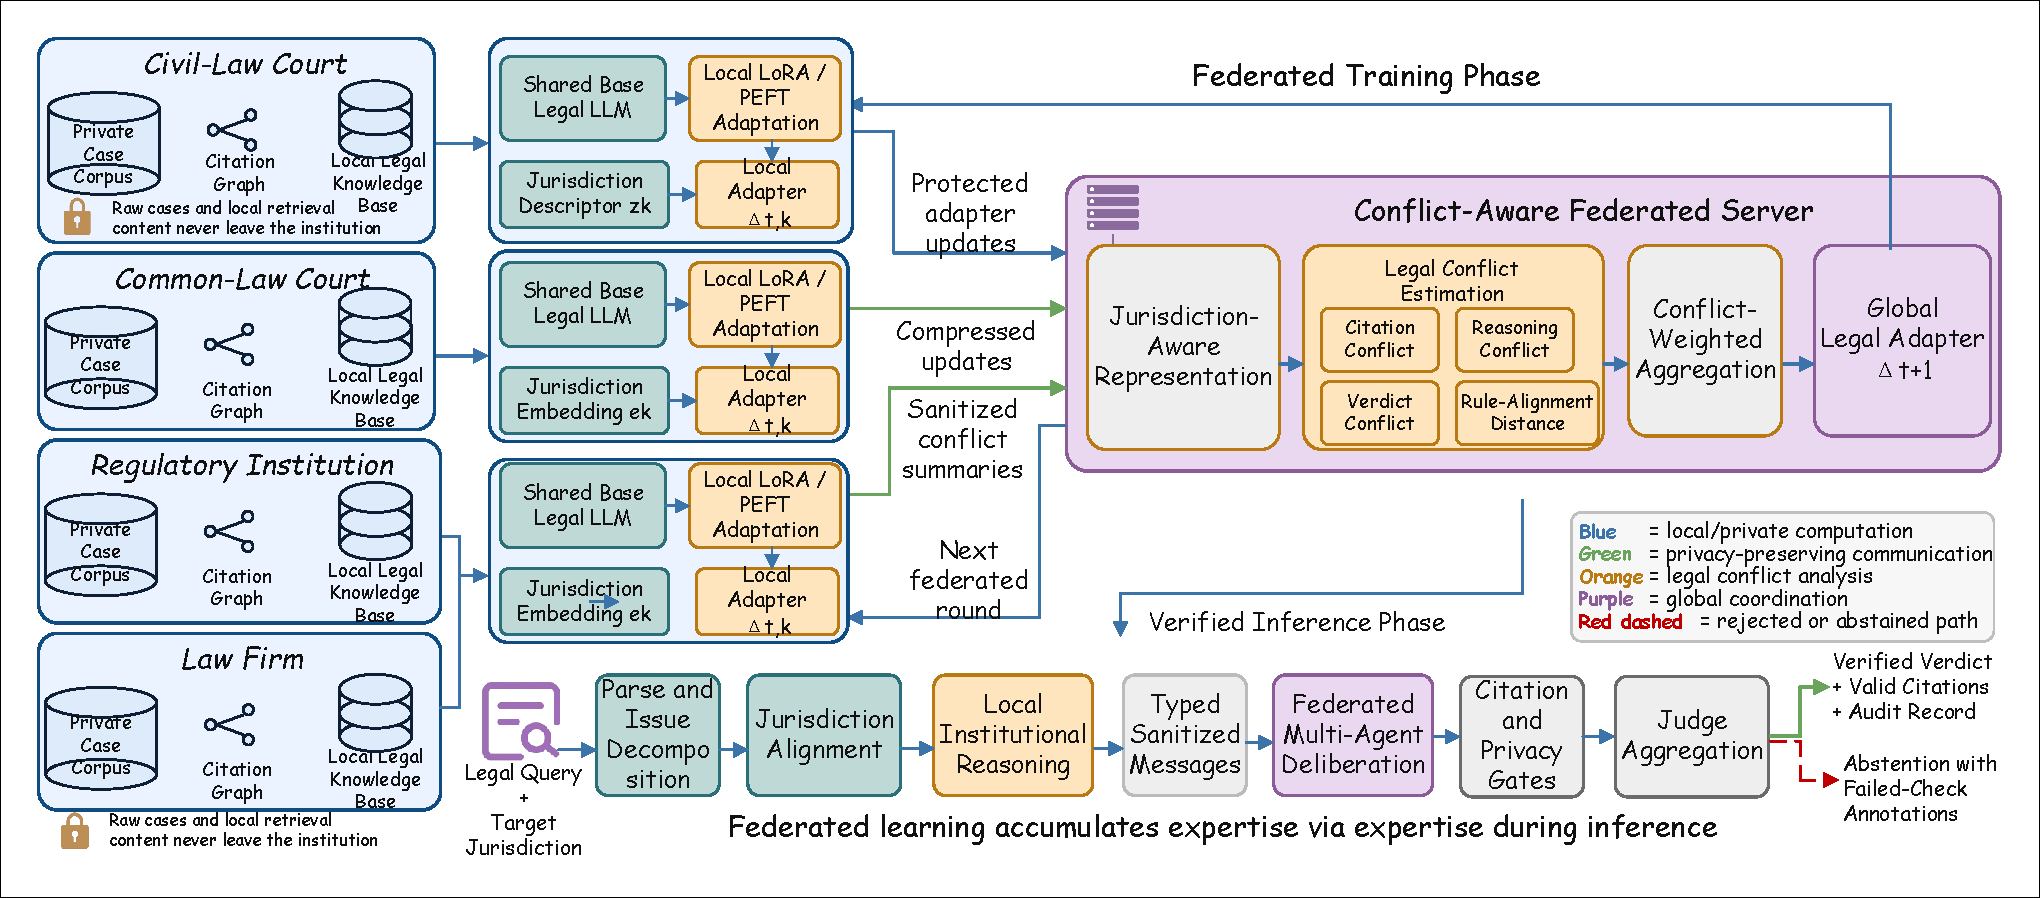
\includegraphics[width=\linewidth]{fig1_flen_architecture.pdf}
    \caption{FLEN: Federated Legal LLM Architecture. Institutions retain raw records and local retrieval state while exchanging configured adapter payloads and minimized probe summaries. The method applies comparability and authority checks before target-conditioned aggregation, retains guarded jurisdiction-local residuals, and gates inference outputs by citation, conflict, and policy status. The CaseHOLD screening exercises the training-time path with automatic proxy metadata; Sections~\ref{sec:privacy-boundary} and~\ref{sec:experiments} define the privacy boundary and report the measured studies.}
    \label{fig:framework}
\end{figure}

Each institution maintains local case corpora, citation graphs, legal knowledge bases, and reasoning trajectories. The design distinguishes jurisdiction, legal domain, language, institution type, and court level rather than treating them as interchangeable client labels. Non-IID simulation may vary topic or label concentration within a task; a cross-jurisdiction experiment additionally requires authentic jurisdiction metadata and a common task or audited output mapping.

Each client adapts Qwen2.5-0.5B-Instruct using LoRA. The measured configuration uses rank 8, scaling factor 16, dropout 0.05, and target modules \texttt{q\_proj} and \texttt{v\_proj}. Payload type is fixed within each controlled comparison. Gradients, adapters, and reasoning embeddings remain distinct communication objects in the system design.

The two paths in Figure~\ref{fig:framework} clarify the complementary roles of federation and agent collaboration. The upper path accumulates jurisdiction-sensitive capability from distributed private experience and broadcasts the global adapter after conflict-aware weighting. The lower path applies that capability to a particular query: institutional outputs are converted into admissible typed messages, challenged through deliberation, and released only after citation and privacy verification. Consequently, the multi-agent layer does not replace federated learning, and the federated server does not directly synthesize an unverified judicial decision.

\subsection{Jurisdiction-aware representation}

Legal non-IID data cannot be represented only by label distributions. We attach a structured descriptor $z_k$ to each client containing jurisdiction, legal domain, language, institution type, court level, and authority hierarchy. In the full method, categorical fields are embedded and concatenated with a text encoding of the documented jurisdiction profile to form $e_k \in \mathbb{R}^{d}$. The descriptor conditions local training and target-jurisdiction routing:
\begin{equation}
    h_i = f_{\theta}(x_i, e_k, r_i),
\end{equation}
where $r_i$ denotes retrieved local legal context and $h_i$ is the case representation used for prediction or reasoning.
The descriptor schema, encoder version, training objective, and missing-value policy are frozen before evaluation. The current pilot uses recorded metadata for routing; jurisdiction-embedding evaluation belongs to the confirmatory protocol.

\subsection{Conflict-aware aggregation}

Standard FedAvg updates a single global model by weighted averaging:
\begin{equation}
    w_{t+1}^{\mathrm{FedAvg}} = \sum_{k=1}^{K}p_k w_{t,k},
    \quad p_k=\frac{n_k}{\sum_{\ell=1}^{K}n_\ell}.
\end{equation}
Unconditional conflict downweighting would suppress a legally valid minority client whenever it disagrees with a larger aligned group. FLEN therefore conditions transfer on a target jurisdiction $j$ and retains a jurisdiction-local residual. Let $\mathcal{E}_{t,k}^{(j)}$ contain valid comparisons involving client $k$ that passed the comparability gate for target $j$. The unresolved conflict exposure is
\begin{equation}
    \delta_{k\rightarrow j}^{(t)} =
    \frac{1}{|\mathcal{E}_{t,k}^{(j)}|}
    \sum_{(k,\ell,q)\in\mathcal{E}_{t,k}^{(j)}}
    D_{\mathrm{conflict}}(k,\ell;q),
\end{equation}
with $\delta_{k\rightarrow j}^{(t)}=0$ when no comparison is admissible. Let $u_{k\rightarrow j}\in[0,1]$ be the frozen target-authority compatibility score and let $n_{\max}$ cap the influence of client size. The normalized base weight is
\begin{equation}
    b_{k\rightarrow j}=
    \frac{u_{k\rightarrow j}\min(n_k,n_{\max})}
    {\sum_{\ell\in\mathcal{G}_j}u_{\ell\rightarrow j}\min(n_\ell,n_{\max})}.
\end{equation}
Citation volume or agreement with a majority is not used as a reliability multiplier unless its calibration is independently validated. A conflict-sensitive candidate weight is
\begin{equation}
    \widehat{\alpha}_{k\rightarrow j}^{(t)} =
    \frac{b_{k\rightarrow j}\exp(-\lambda \delta_{k\rightarrow j}^{(t)})}
    {\sum_{\ell\in\mathcal{G}_j}b_{\ell\rightarrow j}
    \exp(-\lambda \delta_{\ell\rightarrow j}^{(t)})},
\end{equation}
where $\mathcal{G}_j$ is the transfer-compatible cohort. To prevent a feedback loop that eliminates a minority jurisdiction, FLEN mixes this candidate with the base distribution using a diversity floor $\tau\in[0,1]$:
\begin{equation}
    \widetilde{\alpha}_{k\rightarrow j}^{(t)} =
    (1-\tau)\widehat{\alpha}_{k\rightarrow j}^{(t)}
    + \tau b_{k\rightarrow j}.
\end{equation}
For stability, deployed weights use a pre-specified exponential update
\begin{equation}
    \alpha_{k\rightarrow j}^{(t)}=
    (1-\nu)\alpha_{k\rightarrow j}^{(t-1)}
    +\nu\widetilde{\alpha}_{k\rightarrow j}^{(t)},
\end{equation}
followed by normalization within $\mathcal{G}_j$. The smoothing coefficient $\nu$, conflict coefficient $\lambda$, and diversity floor $\tau$ are selected on validation jurisdictions and frozen before held-out-jurisdiction testing. Their sensitivity and the resulting minimum client weight are reported.
The implementation aggregates the shared LoRA factor state $\vartheta_s=(A_s,B_s)$ within the target cohort. Its shared state and effective client-layer weight are
\begin{equation}
    \vartheta_{s,t+1,j}=
    \sum_{k\in\mathcal{G}_j}\alpha_{k\rightarrow j}^{(t)}
    \vartheta_{s,t,k},
    \qquad
    W_{t+1,k}=W_0+s\bigl(B_sA_s+\gamma_k B_kA_k\bigr),
\end{equation}
where $s$ is the LoRA scale. Factor averaging is the shared aggregation rule for the compared PEFT methods; each resulting factor state defines its effective matrix update.
The revised implementation uses two independent LoRA branches with identical target modules. For a layer input $h$, its adapter output is $B_sA_sh+\gamma_k B_kA_kh$, with the usual LoRA scaling and a retained-branch indicator $\gamma_k\in\{0,1\}$. The shared branch is initialized from the target-cohort adapter and trained during the federated phase; its factors alone are uploaded. The private branch persists client-side and is optimized with the shared factors frozen. A deterministic holdout reserved from each client's training shard is excluded from both training phases for every compared method. The private branch is retained when the composed model preserves holdout accuracy and loss; otherwise inference uses the shared branch alone and the private output is reset to zero. External validation and test sets never participate in this selection. Adding two low-rank matrix outputs differs from adding their factors: $(B_s+B_k)(A_s+A_k)$ introduces cross terms. The legacy screening used factor-space residuals; the revised experiments evaluate the independent-branch implementation.
Figure~\ref{fig:conflict-aggregation} illustrates the aggregation mechanism.

\begin{figure}[t]
    \centering
    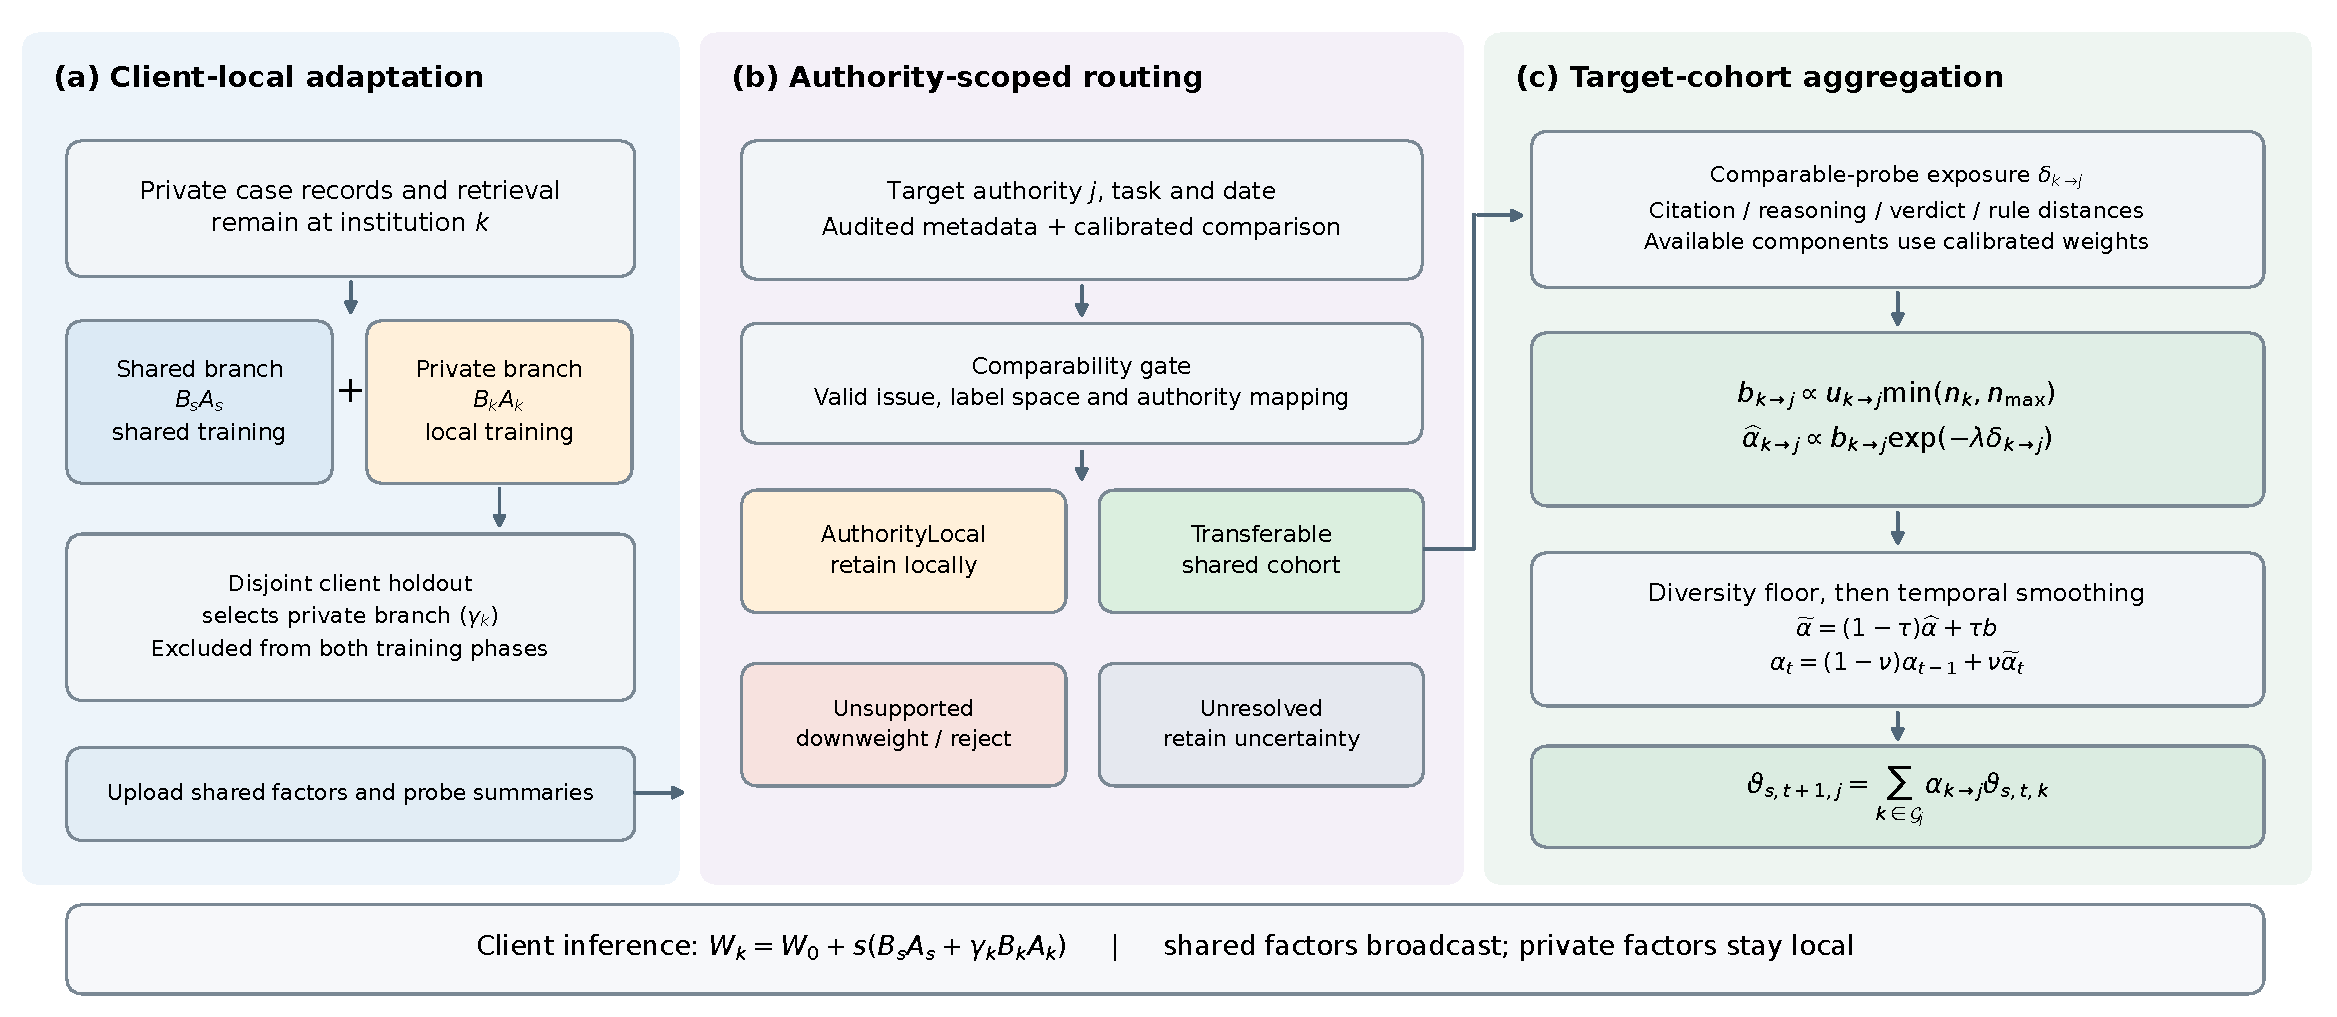
\includegraphics[width=\linewidth]{fig2_operational_conflict_aggregation.pdf}
    \caption{Target-conditioned legal-conflict routing and independent LoRA branches. (a) Shared and private branches have separate factors; the private branch is selected on a disjoint client holdout. (b) Audited authority scope and comparability determine transfer routing. (c) Comparable-probe exposure sets cohort weights, followed by a diversity floor and temporal smoothing. Shared factors are aggregated and broadcast; private factors remain local. The full protocol uses expert-calibrated authority routing, while the screening evaluates automatic proxy exposure.}
    \label{fig:conflict-aggregation}
\end{figure}

Figure~\ref{fig:conflict-aggregation} summarizes the implemented training-time mechanism: conflict measurement is separated from transfer eligibility, incomparable differences remain local, and calibrated proxy conflict inside a target-compatible cohort affects shared transfer. The CaseHOLD screening tests this path with automatic verdict proxies; expert construct validation covers the citation, reasoning, and rule-alignment components.

\begin{algorithm}[t]
\caption{Conflict-aware federated legal LoRA aggregation}
\label{alg:aggregation}
\DontPrintSemicolon
\KwIn{Clients $\client$, target cohorts, probe set, rounds $T$, conflict weight $\lambda$, diversity floor $\tau$}
\KwOut{Target-conditioned shared adapters and jurisdiction-local residuals}
\For{$t=0$ \KwTo $T-1$}{
    Server broadcasts target-cohort adapters, probe identifiers, and the frozen configuration\;
    \ForEach{client $k$ in parallel}{
        Client trains shared factors $\vartheta_{s,t,k}$ on $\dataset_k\setminus H_k$ with the private branch disabled\;
        Client computes available minimized conflict summaries from the shared branch on disjoint probes\;
        Client trains its private branch on $\dataset_k\setminus H_k$ with shared factors frozen\;
        Client selects the private branch on $H_k$ and keeps its factors local\;
        Client sends shared factors and configured probe summaries under the declared threat model\;
    }
    Server computes $D_{\mathrm{cit}},D_{\mathrm{rea}},D_{\mathrm{ver}},D_{\mathrm{rule}}$\;
    Server applies the comparability gate and computes target-conditioned exposure $\delta_{k\rightarrow j}^{(t)}$\;
    Server forms diversity-floored, temporally smoothed weights and aggregates shared factors per target cohort\;
    Server logs communication cost, client drift, aggregation stability, and privacy metrics\;
}
\end{algorithm}

\subsection{Threat model and privacy boundary}
\label{sec:privacy-boundary}

FLEN's implemented baseline provides data locality: raw client records are not intentionally uploaded to the server. Adapters, gradients, verdict distributions, embeddings, summaries, and audit logs remain potential channels for membership, attribute, or text leakage. The policy auditor and \texttt{privacy\_tag} record requested controls and schema-check outcomes; formal protection is defined by the differential-privacy and cryptographic protocol below.

A privacy-preserving instantiation specifies the adversary, protected unit, adjacency relation, clipping norm, sampling rate, noise multiplier, accountant, and final $(\epsilon,\delta)$ after composition. Disclosed probe summaries receive a separate privacy budget or cryptographic computation in addition to update protection. Evaluation includes membership inference, update reconstruction, and embedding-attribute or text-recovery attacks under the utility-reporting protocol.

Secure aggregation also changes the conflict protocol. A compatible two-stage design first computes auditable weights from public probes and differentially private summaries, or through secure multiparty computation; clients then scale their updates by the published weights and securely aggregate the weighted sum. Reporting covers dropout handling, collusion threshold, and protocol overhead. The current pilot implements data-local execution; the formal privacy condition begins when this protocol and its attacks are executed.

\subsection{Federated multi-agent legal reasoning protocol}

The proposed multi-agent workflow is represented as a directed state graph $\graph_A=(V_A,E_A)$. Its state nodes are
\begin{multline*}
V_A = \{\textsc{Parse},\textsc{Align},\textsc{Local},\textsc{Argue},\textsc{Counter},\\
\textsc{Verify},\textsc{Detect},\textsc{Audit},\textsc{Judge}\}.
\end{multline*}
A query moves through typed state transitions rather than unrestricted prompt exchange. A transmitted message has schema
\begin{equation}
    m = (\mathrm{case\_id}, \mathrm{sender}, \mathrm{jurisdiction},
    \mathrm{issue\_ids}, C, \rho, \bm{r}, \bm{\pi}, \mathrm{privacy\_tag}),
\end{equation}
where $C$, $\rho$, $\bm{r}$, and $\bm{\pi}$ are the minimized summaries used by the conflict functions. The \texttt{privacy\_tag} records requested controls and realized budget identifiers. Messages containing raw case text or client-local retrieval content are not admissible on inter-client edges, but the admissible fields remain subject to the leakage analysis in Section~\ref{sec:privacy-boundary}.

The protocol defines three memory scopes. Short-term deliberation memory $M^{\mathrm{case}}$ stores the active issue decomposition, disclosed argument summaries, contradiction flags, and the judge decision for a single query. Jurisdiction memory $M^{\mathrm{jur}}_k$ stores locally maintained rule mappings, authority hierarchies, and alignment metadata for client $k$; only sanitized mappings can be shared. Citation memory $M^{\mathrm{cit}}$ stores canonical citation identifiers, validity results, and authority-level checks required for reproducible citation consistency evaluation. A reasoning trace log records admissible message transitions and verifier decisions for later audit.

The argument and counterargument roles are assigned opposed issue-level analyses conditioned on the aligned jurisdiction state; task-specific labels may specialize them as prosecution/defence, claimant/respondent, or clause/support review. Before synthesis, the citation-verification stage rejects unsupported citations and incompatible authority claims. Conflict detection evaluates pairwise disclosed summaries and records unresolved conflicts. The judge stage receives verified arguments, verdict distributions, conflict scores, and policy-audit status, then emits a final output only when citation, authority, conflict, and privacy-policy gates are satisfied.

\begin{figure}[t]
    \centering
    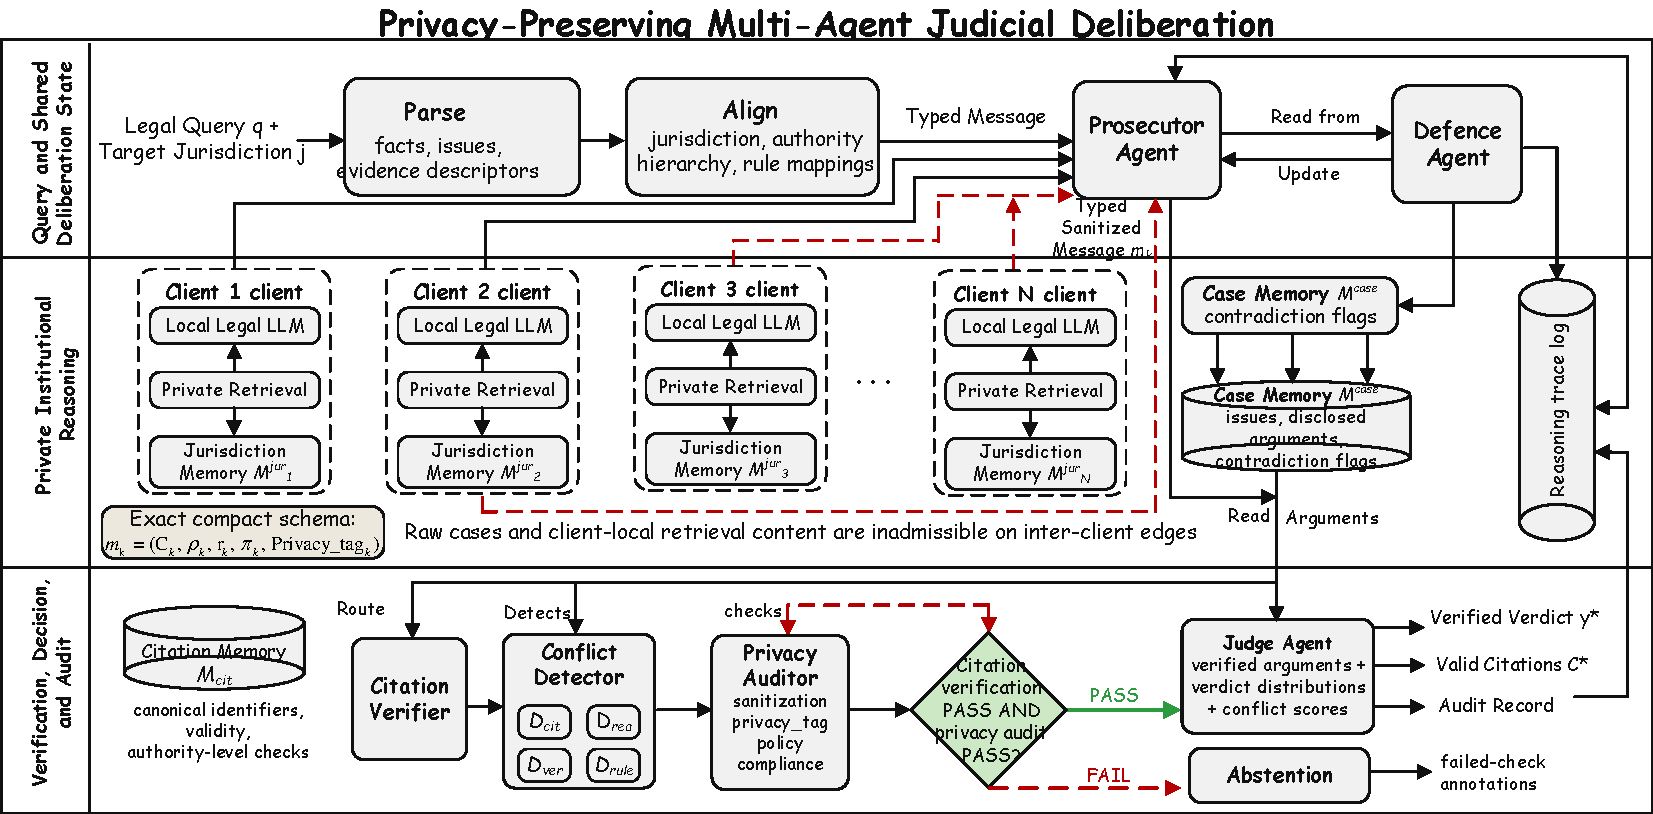
\includegraphics[width=\linewidth]{fig3_privacy_preserving_deliberation.pdf}
    \caption{Proposed policy-gated data-local multi-agent deliberation. The workflow separates shared query state, client-local retrieval, and verification/decision/audit layers. A query is aligned with the target jurisdiction before institutions produce typed minimized messages. Argument and counterargument roles expose competing analyses, while citation, authority, conflict, and policy gates constrain admissible evidence. Formal privacy follows the protocol in Section~\ref{sec:privacy-boundary}.}
    \label{fig:multi-agent}
\end{figure}

Figure~\ref{fig:multi-agent} makes the intended disclosure boundary explicit: private retrieval and jurisdiction memory remain client-local, whereas only schema-constrained messages enter shared deliberation. Case memory coordinates the active arguments, citation memory supports authority validation, and the reasoning trace records admissible transitions and gate outcomes. This separation is designed to let the judge synthesize institution-specific legal expertise without receiving unrestricted raw case content.

\begin{algorithm}[t]
\caption{Policy-gated data-local multi-agent judicial deliberation}
\label{alg:deliberation}
\DontPrintSemicolon
\KwIn{Query $q$, target jurisdiction $j$, local memories $\{M^{\mathrm{jur}}_k\}$}
\KwOut{Verified verdict $y^{*}$ with citations $C^{*}$ and audit record}
\textsc{Parse} extracts issues and sanitized fact descriptors into $M^{\mathrm{case}}$\;
\textsc{Align} retrieves rule mappings and authority levels from $M^{\mathrm{jur}}_j$\;
\ForEach{participating client $k$}{
    \textsc{Local} emits admissible message $m_k=(C_k,\rho_k,\bm{r}_k,\bm{\pi}_k,\mathrm{privacy\_tag}_k)$\;
}
\textsc{Argue} and \textsc{Counter} construct opposed issue-level summaries\;
\textsc{Verify} canonicalizes citations and rejects invalid authority claims\;
\textsc{Detect} computes $D_{\mathrm{cit}},D_{\mathrm{rea}},D_{\mathrm{ver}},D_{\mathrm{rule}}$\;
\textsc{Audit} verifies sanitization and privacy-policy compliance\;
\If{citation, authority, conflict-threshold, and privacy-policy checks pass}{
    \textsc{Judge} aggregates verified summaries and outputs $(y^{*},C^{*})$\;
}
\Else{
    Return an abstention with failed-check annotations\;
}
\end{algorithm}

\FloatBarrier
\section{Experiments}
\label{sec:experiments}

\subsection{Experimental setup}

The evaluation separates optimization, language transfer, privacy, and reasoning. CaseHOLD tests aggregation and personalization under controlled non-IID partitions. MultiEURLEX tests source-to-target language behavior within a shared EU regulatory authority. A client-update privacy study measures membership leakage and utility under replace-one Gaussian protection. Paired CaseHOLD inference compares single-agent prediction with typed four-stage deliberation. The federated studies use Qwen2.5-0.5B-Instruct with matched seeds or paired examples. Run-level means are accompanied by standard deviations; paired differences use 95\% intervals over matched seeds or examples. The completed legacy screenings and privacy study are reported separately from the frozen revision protocol below.

The legacy CaseHOLD comparison includes FedAvg, FedProx, a target-cohort control with $\lambda=0$, conflict-only aggregation, and local-residual variants. The revised comparison adds Ditto and FedAdam~\citep{reddi2021adaptive} and uses independent shared and private LoRA branches. MultiEURLEX compares FedAvg, FedProx, the $\lambda=0$ control, proxy-FLEN, a frozen backbone with a supervised classification head, and a target-supervised local-only reference across four language conditions. The held-out language is excluded from federated threshold selection.

\begin{table}[t]
\caption{Frozen revision protocols. Counts denote scheduled runs or conditions; completed outcomes are identified in the results.}
\label{tab:revision-protocol}
\centering
\small
\begin{tabular}{@{}p{0.19\linewidth}p{0.73\linewidth}@{}}
\toprule
Study & Matched design \\
\midrule
CaseHOLD & Eight conditions $\times$ five seeds; twenty rounds; 1,200 training, 80 validation and 1,000 fixed test records; independent shared/private LoRA branches. \\
FedAdam & Five additional seeds; same ten-step clients as FedAvg; Flower adaptive server optimizer. \\
MultiEURLEX & Six methods $\times$ four holdouts $\times$ five seeds; three rounds; 500 training records and 64 separate probes per source client; 500 validation and 500 fixed test records per language. \\
Privacy & Five conditions $\times$ three seeds; unclipped, clipping-only and three noise levels; disjoint source probes and threshold validation. \\
LegalBench & Four tasks; 492 fixed cases; two pretrained checkpoints plus five FedAvg and five FLEN shared adapters. \\
Reasoning & Three checkpoints $\times$ two single-agent call budgets; same sixty cases; four-stage deliberation and blinded presentation. \\
\bottomrule
\end{tabular}
\end{table}


All federated adapters use rank eight, scaling sixteen, and query/value projections. CaseHOLD uses AdamW at $2\times10^{-4}$, batch size one, accumulation over four batches, and a 512-token limit. MultiEURLEX uses AdamW at $2\times10^{-5}$, batch size four, a 256-token limit, and one local epoch per round, jointly training the classification head. CaseHOLD selects the holding with the smallest mean answer-token loss; MultiEURLEX applies a validation-selected threshold to 21 sigmoid label outputs.

\paragraph{Frozen tests and matched contrasts.}
The revised CaseHOLD study fixes 1,000 test records before training and evaluates them after round twenty. Four equal, fixed test shards define deployment clients. Guarded and unguarded personalization are compared at both $8+2$ and $10+2$ shared/private optimizer steps, with identical gate records excluded from both training phases. FedAdam uses the same ten-step clients as FedAvg and the Flower server optimizer with learning rate 0.01, $\beta_1=0.9$, $\beta_2=0.99$, and $\tau=10^{-9}$. Five matched training seeds determine run-level uncertainty. Paired Student-$t$ intervals describe effect magnitude; exact two-sided sign-flip tests and Holm adjustment are reported for planned contrasts within each metric. With five pairs, the smallest attainable two-sided sign-flip $p$-value is 0.0625.

The revised MultiEURLEX matrix uses the same 500 test records per language across methods and training seeds. Each source client reserves 64 additional training-split records as aggregation probes, separate from the 500-record validation sample used for threshold selection. Test predictions are produced after the final round. For method $m$ and seed $s$, average and worst held-out-language micro-$F_1$ are computed as
\begin{equation}
 \bar F_{m,s}=\frac{1}{4}\sum_{\ell=1}^{4}F_{m,s,\ell},
 \qquad F^{\min}_{m,s}=\min_{\ell\in\{1,\ldots,4\}} F_{m,s,\ell}.
\end{equation}
Uncertainty and paired method differences are then calculated over training seeds. Thresholds at the search boundary remain in the analysis. Local-only adaptation uses target-language labels and is reported as a target-supervised reference.

\paragraph{Published-label component diagnostics.}
A separate LegalBench~\citep{guha2023legalbench} protocol tests precedent overruling, UCC versus common-law applicability, citation support, and personal jurisdiction. A fixed sample contains 240, 94, 108, and 50 test cases, respectively. Each prompt supplies the legal material and allowed labels; citation classification also supplies the proposed citation. Labels are scored by mean answer-token negative log likelihood. The protocol compares the pretrained Qwen backbone with five FedAvg and five FLEN shared adapters, and includes pretrained Mistral-7B-Instruct-v0.2 as a larger-model reference. Accuracy, macro-$F_1$, balanced accuracy, multiclass Brier score, and ten-bin confidence ECE describe distinct outcomes. Adapter effects are paired across training seeds; the pretrained-reference contrast is paired across cases. These tasks measure benchmark components, while expert authority-pair annotation evaluates the legal-conflict construct.

\paragraph{Inference and resource controls.}
The revised reasoning protocol crosses base, FedAvg-shared, and FLEN-shared checkpoints with one-call and four-call single-agent controls and four-stage deliberation on the same sixty cases. The four-call control repeatedly rechecks its answer against the supplied holdings. Analysis prompt tokens, generated tokens, and elapsed time are recorded separately from the shared presentation step. A repeated deterministic four-stage output is counted once per checkpoint. Case-level bootstrap intervals and exact McNemar tests quantify prediction differences; the seed-41 checkpoint comparison measures those checkpoints. Logical federated payload and client drift accompany task performance. Elapsed times are interpreted alongside recorded GPU metadata.

\IfFileExists{sections/revision_casehold_results.tex}{%
\subsection{Matched-budget dual-branch revision}
The completed revision evaluates forty original configurations and five additional FedAdam runs. All runs use independent final-test predictions and the frozen training schedule. Worst-client accuracy is reconstructed from saved predictions using the same four round-robin test shards for every run; early shared-only runs originally logged a different grouping. Table~\ref{tab:revision-casehold} reports aggregate and worst-client outcomes.

\begin{table}[t]
\caption{Independent dual-LoRA revision: five seeds, twenty rounds and 1,000 fixed test records. Accuracy entries are percent mean and seed SD; time is observed mean wall minutes.}
\label{tab:revision-casehold}
\centering
\small
\resizebox{\linewidth}{!}{%
\begin{tabular}{lrrrr}
\toprule
Method (shared+private) & Accuracy & Worst client & Fit payload (MiB) & Minutes \\
\midrule
FedAvg (10) & 28.28 $\pm$ 0.77 & 26.80 $\pm$ 0.80 & 330.00 & 15.3 \\
FedProx (10) & 28.34 $\pm$ 1.09 & 26.40 $\pm$ 1.26 & 330.00 & 14.9 \\
Ditto (8+2) & 25.60 $\pm$ 0.70 & 22.48 $\pm$ 1.18 & 330.00 & 17.4 \\
Unguarded (8+2) & 25.28 $\pm$ 1.13 & 21.20 $\pm$ 2.06 & 330.01 & 40.1 \\
Guarded (8+2) & 27.78 $\pm$ 1.42 & 26.00 $\pm$ 1.52 & 330.01 & 38.0 \\
Unguarded (10+2) & 25.92 $\pm$ 1.55 & 22.32 $\pm$ 1.73 & 330.01 & 40.1 \\
Guarded (10+2) & 28.56 $\pm$ 1.03 & 26.40 $\pm$ 0.98 & 330.01 & 39.6 \\
Proxy-FLEN (8+2) & 27.84 $\pm$ 1.40 & 25.76 $\pm$ 1.56 & 330.01 & 38.7 \\
FedAdam (10) & 21.28 $\pm$ 0.61 & 18.96 $\pm$ 1.15 & 330.00 & 13.2 \\
\bottomrule
\end{tabular}
}
\end{table}


At the $8+2$ budget, gating changes accuracy by $+2.50$ points (95\% paired interval $[1.63,3.37]$). At $10+2$, its effect is $+2.64$ points (95\% paired interval $[1.60,3.68]$). Adding proxy conflict weights to guarded $8+2$ changes accuracy by $+0.06$ points (95\% paired interval $[-0.42,0.54]$). These fixed-budget contrasts separate private selection from additional shared optimization.

The two gate effects are positive across all five seed pairs. Their exact two-sided sign-flip $p$-values are 0.0625, with Holm-adjusted $p=0.4375$ across seven planned accuracy contrasts. The intervals quantify recovery relative to unguarded adaptation; the small seed count limits exact-test resolution. Guarded $8+2$ accuracy is 27.78\%, compared with 28.28\% for FedAvg and 28.34\% for FedProx. FedAdam reaches 21.28\% at the fixed server setting; its hyperparameters were not optimized on these test outcomes.

\begin{table}[t]
\caption{Private-branch diagnostics. Acceptance is the fraction of client-round candidates retained; the final test gain compares the selected composition with the shared branch, in percentage points.}
\label{tab:revision-gate}
\centering
\small
\begin{tabular}{lrr}
\toprule
Method & Accepted (percent) & Private minus shared \\
\midrule
Unguarded (8+2) & 100.00 $\pm$ 0.00 & -2.30 $\pm$ 1.05 \\
Guarded (8+2) & 39.75 $\pm$ 10.44 & 0.00 $\pm$ 0.00 \\
Unguarded (10+2) & 100.00 $\pm$ 0.00 & -2.74 $\pm$ 0.68 \\
Guarded (10+2) & 35.50 $\pm$ 5.97 & 0.16 $\pm$ 0.17 \\
Proxy-FLEN (8+2) & 38.25 $\pm$ 11.44 & 0.04 $\pm$ 0.09 \\
\bottomrule
\end{tabular}
\end{table}


The gate retains 39.75\% and 35.50\% of client-round candidates at the two budgets. The selected private branch changes final accuracy relative to its shared branch by 0.00 and 0.16 points, respectively; unguarded private branches reduce it by 2.30 and 2.74 points. Thus the main observed benefit is removal of harmful private updates, while the retained private branch contributes little additional test utility.

\begin{figure}[t]
\centering
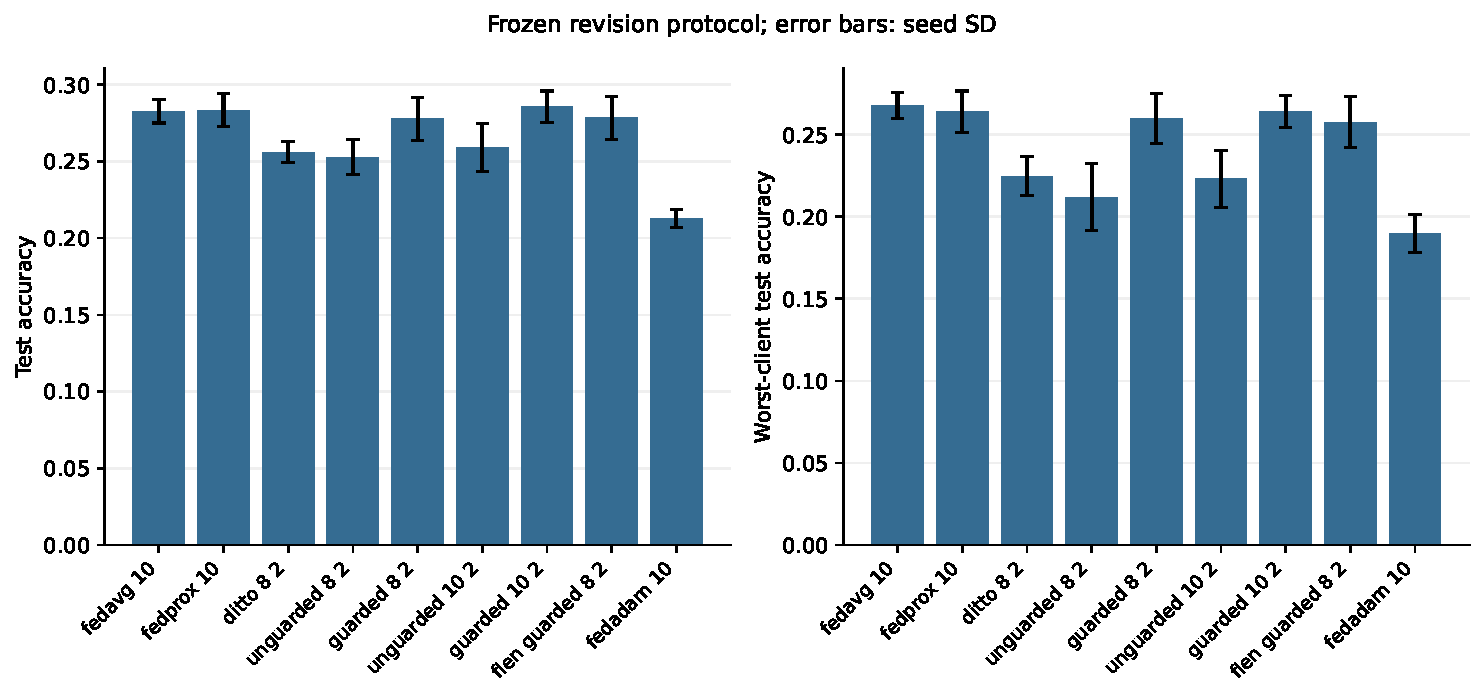
\includegraphics[width=\linewidth]{revision_casehold.pdf}
\caption{Completed dual-branch revision. Bars show five-seed means and seed SD on fixed test records. Worst client denotes a fixed test shard.}
\label{fig:revision-casehold}
\end{figure}

}{%
\subsection{Legacy CaseHOLD mechanism and ablation study}

The legacy CaseHOLD study uses four clients, 1,200 training records, 240 validation records, 24 disjoint aggregation probes, and twenty Flower rounds. All 24 runs completed the configured rounds and client evaluations. These runs use a factor-space local residual, whereas the revised method uses independent LoRA branches. Unguarded variants allocate eight shared and two local steps; guarded variants allocate ten shared and two local steps. Their recovery contrast therefore combines a gate change with a shared-training-budget change. Target-conditioned runs record client predictions, proxy conflict exposure, aggregation weights, local-residual decisions, and communication volume. Client labels are heuristic non-IID cohorts, and calibration uses automatic proxy labels.

Table~\ref{tab:e1-flen-screening} reports eight legacy variants. Conflict-only aggregation reaches $35.42\%\pm3.56$ aggregate accuracy, compared with $33.89\%\pm5.75$ for its $\lambda=0$ control; the paired mean difference is $+1.53$ points with a 95\% Student-$t$ interval of $[-8.84,11.90]$. The unguarded $8+2$ shared/local schedule degrades aggregate accuracy by 8.61 points relative to the target-cohort control. Paired client evaluation identifies an adverse local-residual contribution: personalized-minus-shared accuracy averages $-8.19$ points. The guarded $10+2$ configuration reaches $35.56\%\pm3.94$, or $+1.67$ points over $\lambda=0$, while its residual contribution averages $+0.42$ points. The interval for the full comparison is $[-4.80,8.13]$, and guarded FLEN's mean worst-client accuracy is 1.67 points below the control. These results identify adverse personalization and recovery under a combined gate-and-budget change; the revised matched-budget experiment isolates the gate contribution.

All target-conditioned methods communicate $330.01$~MiB of logical model and probe payload per seed, compared with $330.00$~MiB for FedAvg and FedProx. The 0.01~MiB difference is the probe-summary payload. These totals cover logical model traffic before serialization and transport overhead.

\begin{table*}[t]
\caption{Legacy factor-residual CaseHOLD screening over seeds 41--43. Values are mean $\pm$ run-level standard deviation. Unguarded variants use 8+2 shared/local steps, guarded variants use 10+2. ``Aggregated'' is sample-weighted client evaluation on heuristic cohorts.}
\label{tab:e1-flen-screening}
\centering
\resizebox{\textwidth}{!}{%
\begin{tabular}{lrrrrl}
\toprule
Method & Aggregated accuracy $\uparrow$ & Worst-client accuracy $\uparrow$ & Mean update norm & Logical payload (MiB) & Experimental role \\
\midrule
FedAvg & $33.75 \pm 3.15$ & $28.33 \pm 4.41$ & $0.4170$ & $330.00$ & shared baseline \\
FedProx & $34.58 \pm 2.73$ & $30.00 \pm 1.67$ & $0.3635$ & $330.00$ & proximal baseline \\
Target cohort ($\lambda=0$) & $33.89 \pm 5.75$ & $28.89 \pm 8.55$ & $0.4172$ & $330.01$ & target-conditioned control \\
Conflict only & $35.42 \pm 3.56$ & $30.00 \pm 6.67$ & $0.4172$ & $330.01$ & conflict-weight ablation \\
Personalization only, unguarded & $25.56 \pm 1.68$ & $20.00 \pm 1.67$ & $0.3740$ & $330.01$ & residual ablation \\
FLEN, unguarded & $25.28 \pm 2.55$ & $20.00 \pm 4.41$ & $0.3739$ & $330.01$ & budget-matched full variant \\
Personalization only, guarded & $35.14 \pm 2.84$ & $31.67 \pm 5.00$ & $0.4173$ & $330.01$ & residual-safeguard control \\
FLEN, guarded & $35.56 \pm 3.94$ & $27.22 \pm 8.22$ & $0.4172$ & $330.01$ & guarded full variant \\
\bottomrule
\end{tabular}
}
\end{table*}


\begin{figure*}[t]
    \centering
    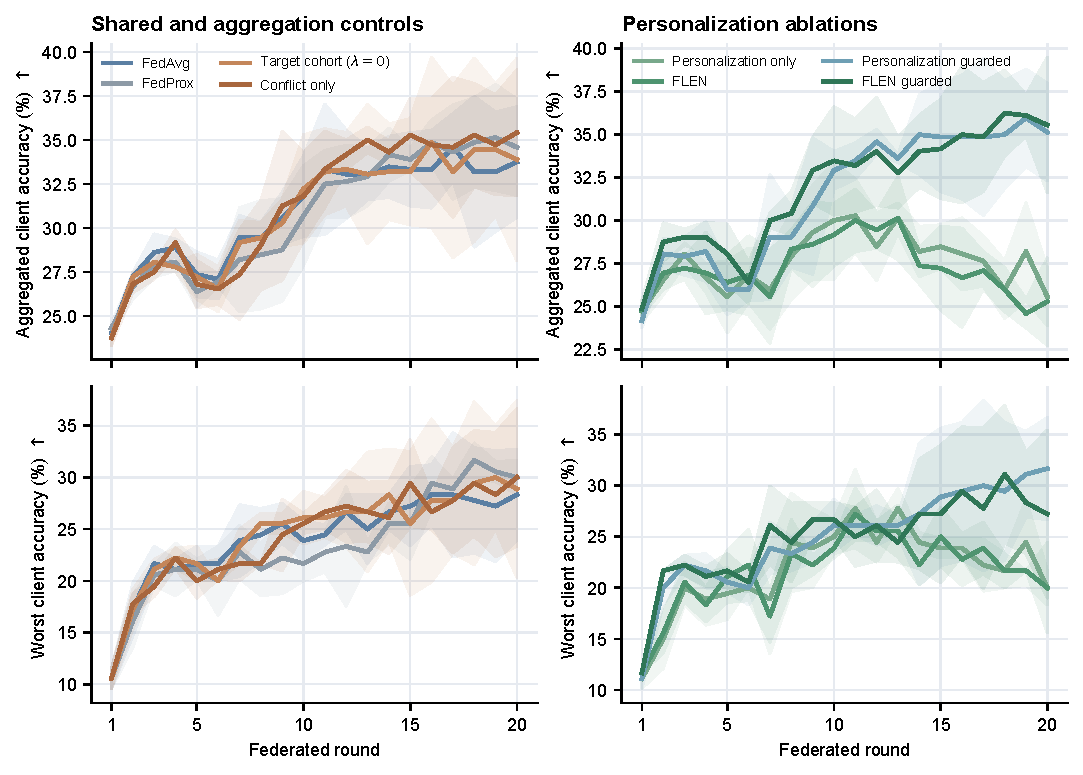
\includegraphics[width=0.96\textwidth]{e1_accuracy_convergence.pdf}
    \caption{Twenty-round legacy CaseHOLD proxy-screening convergence. Curves are means across seeds 41--43 and shaded regions are one standard deviation. The unguarded $8+2$ configuration degrades, while the guarded $10+2$ configuration recovers performance. This comparison changes both the gate and shared-training budget. Client identifiers denote heuristic non-IID cohorts.}
    \label{fig:e1-accuracy-convergence}
\end{figure*}

\begin{figure*}[t]
    \centering
    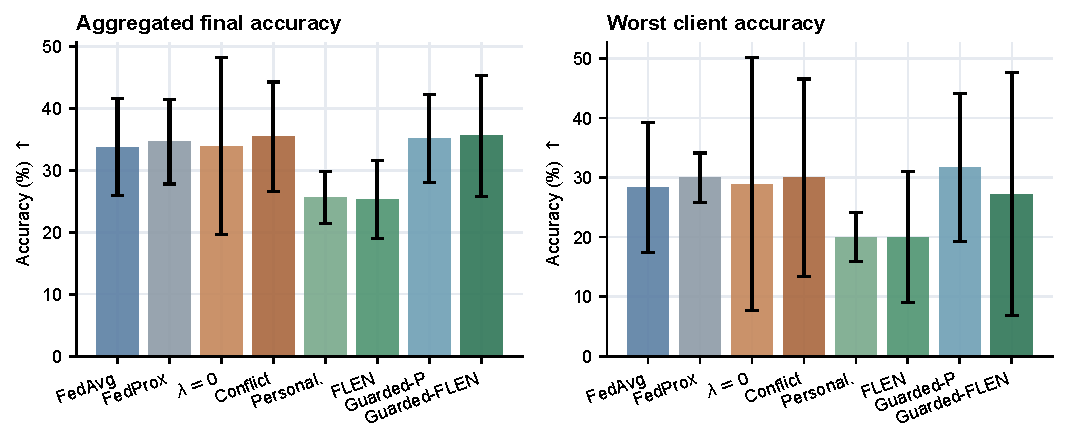
\includegraphics[width=0.90\textwidth]{e1_final_accuracy.pdf}
    \caption{Final aggregate and worst-client CaseHOLD accuracy. Bars report seed means and error bars report 95\% Student-$t$ intervals over three runs. Comparative intervals cross zero, and worst-client means favor the $\lambda=0$ control over guarded FLEN.}
    \label{fig:e1-final-accuracy}
\end{figure*}

\begin{figure*}[t]
    \centering
    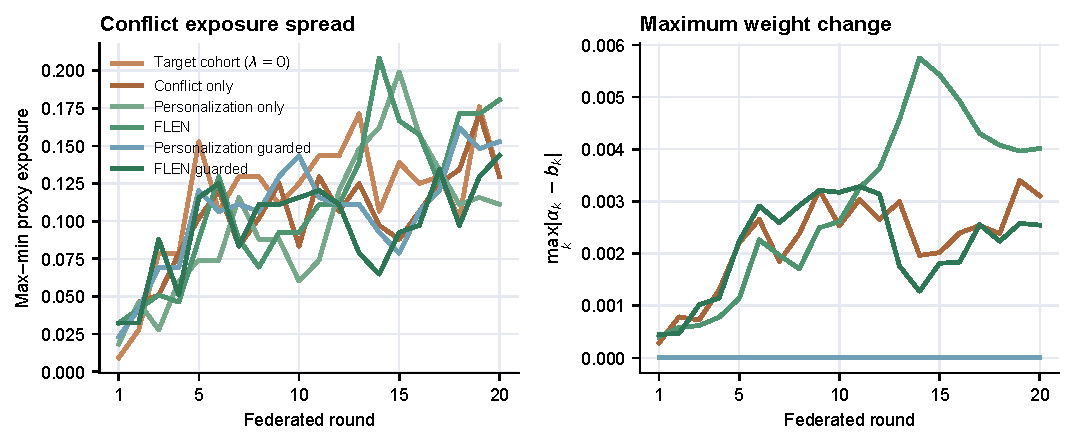
\includegraphics[width=0.96\textwidth]{e1_conflict_diagnostics.pdf}
    \caption{Proxy-conflict mechanism diagnostics. The left panel shows non-uniform gold-error-gated verdict exposure; the right panel shows the maximum absolute change from target-cohort base weights. The $\lambda=0$ controls retain their base weights, while conflict-enabled variants change client weights during training.}
    \label{fig:e1-conflict-diagnostics}
\end{figure*}

\FloatBarrier

}
\IfFileExists{sections/revision_multieurlex_results.tex}{%
\subsection{Disjoint-probe multilingual revision}
The completed six-method, four-holdout, five-seed revision uses fixed test records and separate training probes and threshold-validation examples. Table~\ref{tab:revision-multieurlex} reports language-average and worst-language outcomes.

\begin{table}[t]
\caption{Completed 120-run language-transfer revision. Each seed contributes a mean and minimum across four independently held-out target languages; entries report mean and seed SD.}
\label{tab:revision-multieurlex}
\centering
\small
\resizebox{\linewidth}{!}{%
\begin{tabular}{lrrrr}
\toprule
Method & Mean micro F1 & Worst micro F1 & Macro F1 & Brier \\
\midrule
FedAvg & 0.337 $\pm$ 0.015 & 0.273 $\pm$ 0.037 & 0.168 $\pm$ 0.010 & 0.184 $\pm$ 0.006 \\
FedProx & 0.335 $\pm$ 0.014 & 0.272 $\pm$ 0.037 & 0.167 $\pm$ 0.010 & 0.185 $\pm$ 0.006 \\
$\lambda=0$ & 0.337 $\pm$ 0.015 & 0.273 $\pm$ 0.037 & 0.168 $\pm$ 0.010 & 0.184 $\pm$ 0.006 \\
Proxy-FLEN & 0.336 $\pm$ 0.017 & 0.276 $\pm$ 0.036 & 0.169 $\pm$ 0.009 & 0.185 $\pm$ 0.006 \\
Local only (target labels) & 0.468 $\pm$ 0.011 & 0.449 $\pm$ 0.013 & 0.163 $\pm$ 0.011 & 0.121 $\pm$ 0.001 \\
Frozen backbone + head & 0.310 $\pm$ 0.013 & 0.256 $\pm$ 0.037 & 0.163 $\pm$ 0.009 & 0.214 $\pm$ 0.016 \\
\bottomrule
\end{tabular}
}
\end{table}


Relative to FedAvg, proxy-FLEN changes average micro-$F_1$ by $-0.11$ points (95\% paired interval $[-0.64,0.43]$) and worst-language micro-$F_1$ by $+0.30$ points (95\% paired interval $[-0.13,0.73]$). The frozen-backbone reference changes average micro-$F_1$ by $-2.68$ points (95\% paired interval $[-3.96,-1.41]$); target-supervised local-only adaptation changes it by $+13.06$ points (95\% paired interval $[11.91,14.21]$). The zero-conflict control reproduces FedAvg. Proxy-FLEN's average contrast spans zero, so the study provides no stable incremental benefit from proxy conflict weighting. Target-language supervision remains substantially stronger than three-round source-language transfer. The frozen-backbone reference trains a classification head and therefore measures the contribution of backbone adaptation.

\begin{figure}[t]
\centering
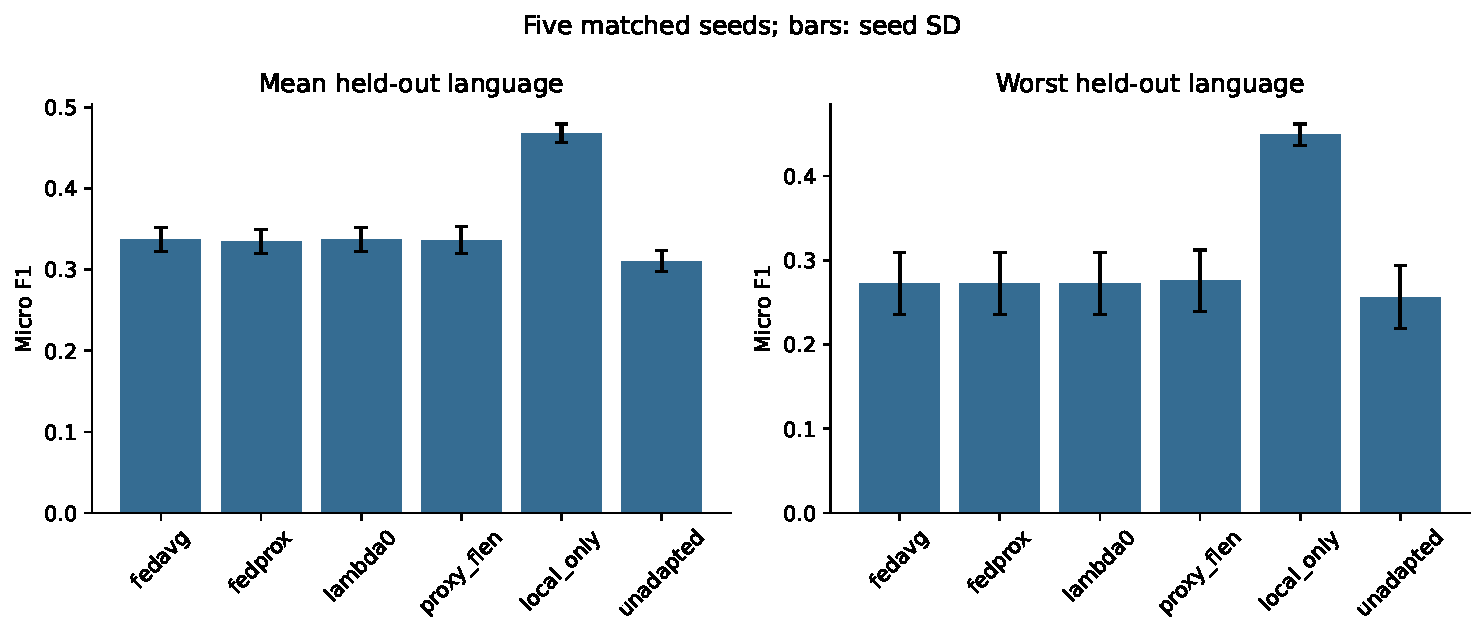
\includegraphics[width=\linewidth]{revision_multieurlex.pdf}
\caption{Mean and worst held-out-language performance in the completed revision; error bars show five-seed SD.}
\label{fig:revision-multieurlex}
\end{figure}

}{%
\subsection{Legacy MultiEURLEX multilingual screening}

The MultiEURLEX study uses English--German, English--French, English--Spanish, and English--Polish language clients. For each held-out pair, the remaining three clients train a LoRA adapter for three rounds using 500 training examples per client. The comparison adds an unadapted backbone with a trained classifier head and local-only adaptation using 500 target-language examples. The local-only condition measures target-supervised adaptation, while the federated conditions measure source-to-target transfer. Evaluation uses 500 validation and 500 test examples per language and matched seeds 41--43. The 72-run matrix completed on GPU and passed method-specific checks for finite metrics, threshold calibration, prediction reconstruction, identifiers, communication accounting, and artifact completeness.

\begin{table*}[t]
\caption{Three-round MultiEURLEX screening with matched seeds 41--43. Values are mean $\pm$ standard deviation. Local-only uses target-language supervision and serves as a target-data reference; the federated methods train on the other three language clients. All clients share the EU regulatory authority scope.}
\label{tab:multieurlex-results}
\centering
\resizebox{\textwidth}{!}{%
\begin{tabular}{lcccccc}
\toprule
Method & DE micro-$F_1$ & FR micro-$F_1$ & ES micro-$F_1$ & PL micro-$F_1$ & Mean micro-$F_1$ & Mean macro-$F_1$ \\
\midrule
FedAvg & $0.2944\pm0.0418$ & $0.4089\pm0.0523$ & $0.2996\pm0.0489$ & $0.3411\pm0.0398$ & $0.3360\pm0.0033$ & $0.1659\pm0.0004$ \\
FedProx & $0.2937\pm0.0419$ & $0.3967\pm0.0534$ & $0.3076\pm0.0398$ & $0.3399\pm0.0386$ & $0.3345\pm0.0060$ & $0.1648\pm0.0059$ \\
$\lambda=0$ control & $0.2944\pm0.0418$ & $0.4089\pm0.0523$ & $0.2996\pm0.0489$ & $0.3411\pm0.0398$ & $0.3360\pm0.0033$ & $0.1659\pm0.0004$ \\
Proxy-FLEN & $0.2990\pm0.0426$ & $0.4014\pm0.0618$ & $0.3065\pm0.0356$ & $0.3425\pm0.0433$ & $0.3373\pm0.0085$ & $\mathbf{0.1695\pm0.0091}$ \\
\midrule
Unadapted backbone & $0.2656\pm0.0209$ & $0.3614\pm0.0102$ & $0.2843\pm0.0492$ & $0.3117\pm0.0180$ & $0.3057\pm0.0123$ & $0.1613\pm0.0077$ \\
Local-only target reference & $\mathbf{0.4686\pm0.0282}$ & $\mathbf{0.4704\pm0.0294}$ & $\mathbf{0.4672\pm0.0254}$ & $\mathbf{0.4337\pm0.0259}$ & $\mathbf{0.4600\pm0.0234}$ & $0.1616\pm0.0073$ \\
\bottomrule
\end{tabular}
}
\end{table*}


FedProx matches FedAvg within uncertainty in Table~\ref{tab:multieurlex-results}. Averaging the four held-out-language scores within each seed, FedProx changes micro-$F_1$ by $-0.0015$ (95\% Student-$t$ interval $[-0.0107,0.0077]$). Legacy proxy-FLEN uses gold-error-gated prediction disagreement on source-language validation probes; those records also contribute to threshold selection. It changes client weights by approximately 0.06 from minimum to maximum per round, with a paired micro-$F_1$ effect over FedAvg of $+0.0013$ ($[-0.0154,0.0181]$). The revised matrix separates probes from threshold-validation records. The $\lambda=0$ control exactly reproduces FedAvg, verifying the control implementation. Each federated run communicates 12.81~MiB per round, or 38.42~MiB over three rounds; local-only communication is zero.

The unadapted reference averages $0.3057$ micro-$F_1$, compared with $0.3360$ for FedAvg; the paired difference is $-0.0303$ with a 95\% interval of $[-0.0581,-0.0024]$, showing that adaptation contributes measurable utility. The target-supervised local-only reference reaches $0.4600$ and exceeds FedAvg by $0.1240$ ($[0.0712,0.1767]$). Source-language federation therefore improves over the unadapted reference but does not match target-language supervision in this three-round setting.

\begin{figure}[t]
    \centering
    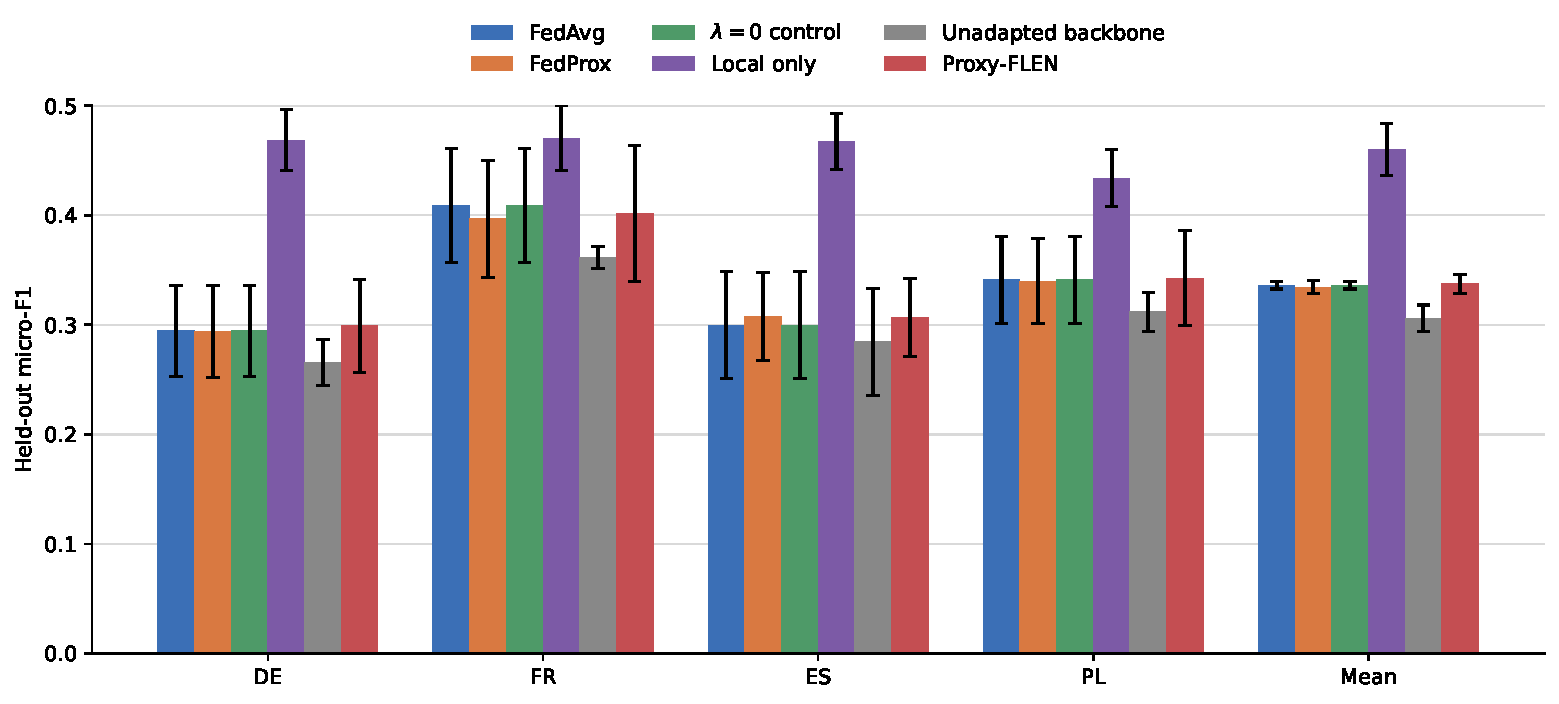
\includegraphics[width=\linewidth]{multieurlex_heldout_micro_f1.pdf}
    \caption{MultiEURLEX micro-$F_1$ over seeds 41--43; error bars show one standard deviation. Local-only uses target-language supervision, whereas the federated methods transfer from the other language clients. Proxy-FLEN activates non-uniform weights but does not improve consistently over FedAvg.}
    \label{fig:multieurlex-heldout}
\end{figure}

\FloatBarrier

}
\subsection{Client-update privacy and membership inference}

The completed privacy revision compares unclipped training, clipping only, and Gaussian noise multipliers 0.25, 0.5, and 1.0 over seeds 41--43, giving 15 runs. It uses replace-one-client-update adjacency, an $L_2$ clipping norm of 1.0, full participation by three source-language clients, and a central Gaussian mechanism on the weighted aggregate. The mechanism assumes a trusted aggregator and protects the released update. The accountant reports the composed three-round $(\epsilon,\delta)$ budget at $\delta=10^{-5}$. Source-training probes are separated from threshold-validation records; final task evaluation uses held-out test records. A black-box loss attack compares source-language training members with source-language test non-members, separating attack calibration and evaluation halves. Its direction and threshold are selected on the calibration half. This diagnostic measures record membership, while the mechanism's protected unit is the client update.

\begin{table*}[t]
\caption{Completed 15-run MultiEURLEX privacy revision over seeds 41--43. Held-out English--Polish results are means $\pm$ seed standard deviations. ECE pools binary label probabilities into 15 bins. The trusted-aggregator client-update accountant uses $\delta=10^{-5}$; the attack measures record membership.}
\label{tab:privacy-attack}
\centering
\resizebox{\textwidth}{!}{%
\begin{tabular}{lrrrrrrr}
\toprule
Condition & $\epsilon$ & Micro-$F_1$ $\uparrow$ & Macro-$F_1$ $\uparrow$ & BCE $\downarrow$ & Brier $\downarrow$ & ECE $\downarrow$ & Attack AUC $\downarrow$ \\
\midrule
Unclipped & -- & $0.341 \pm 0.039$ & $0.184 \pm 0.026$ & $0.73 \pm 0.04$ & $0.222 \pm 0.012$ & $0.211 \pm 0.050$ & $0.617 \pm 0.021$ \\
Clipping only & -- & $0.336 \pm 0.039$ & $0.181 \pm 0.026$ & $0.75 \pm 0.04$ & $0.227 \pm 0.013$ & $0.220 \pm 0.051$ & $0.615 \pm 0.021$ \\
Gaussian $0.25$ & 59.51 & $0.264 \pm 0.058$ & $0.196 \pm 0.051$ & $15.17 \pm 5.71$ & $0.488 \pm 0.060$ & $0.489 \pm 0.060$ & $0.591 \pm 0.039$ \\
Gaussian $0.5$ & 23.51 & $0.250 \pm 0.046$ & $0.206 \pm 0.048$ & $20.70 \pm 5.65$ & $0.481 \pm 0.041$ & $0.481 \pm 0.041$ & $0.525 \pm 0.040$ \\
Gaussian $1.0$ & 9.84 & $0.249 \pm 0.051$ & $0.210 \pm 0.041$ & $36.78 \pm 10.68$ & $0.479 \pm 0.060$ & $0.479 \pm 0.059$ & $0.543 \pm 0.053$ \\
\bottomrule
\end{tabular}
}
\end{table*}


Table~\ref{tab:privacy-attack} separates the clipping and noise effects. Clipping alone changes micro-$F_1$ from 0.341 to 0.336; the paired difference is $-0.0056$ with a 95\% Student-$t$ interval of $[-0.0173,0.0061]$. At $\sigma=0.5$, attack AUC is 0.525, compared with 0.615 for clipping only; its paired difference is $-0.0901$ ($[-0.2145,0.0343]$). The corresponding micro-$F_1$ means are 0.250 and 0.336, while macro-$F_1$ rises from 0.181 to 0.206. The record-membership diagnostic therefore shows an uncertain attack reduction alongside differing task-metric responses.

Probability quality deteriorates strongly under noise. At $\sigma=0.5$, BCE rises from 0.75 to 20.70 and Brier score from 0.227 to 0.481 relative to clipping only; the paired Brier increase is 0.2544 ($[0.1448,0.3639]$). Pooled binary-label ECE rises from 0.220 to 0.481, a paired increase of 0.2615 ($[0.0563,0.4666]$). Figure~\ref{fig:privacy-reliability} shows overconfident predictions across the noisy conditions. At $\sigma=1.0$, attack AUC is 0.543 and BCE is 36.78, so the attack diagnostic does not improve monotonically with noise in this three-seed screen. All completed runs enter the analysis, including boundary-threshold runs. These findings characterize a poor probability-quality regime for the tested small-client, high-dimensional adapter mechanism.

\begin{figure}[t]
    \centering
    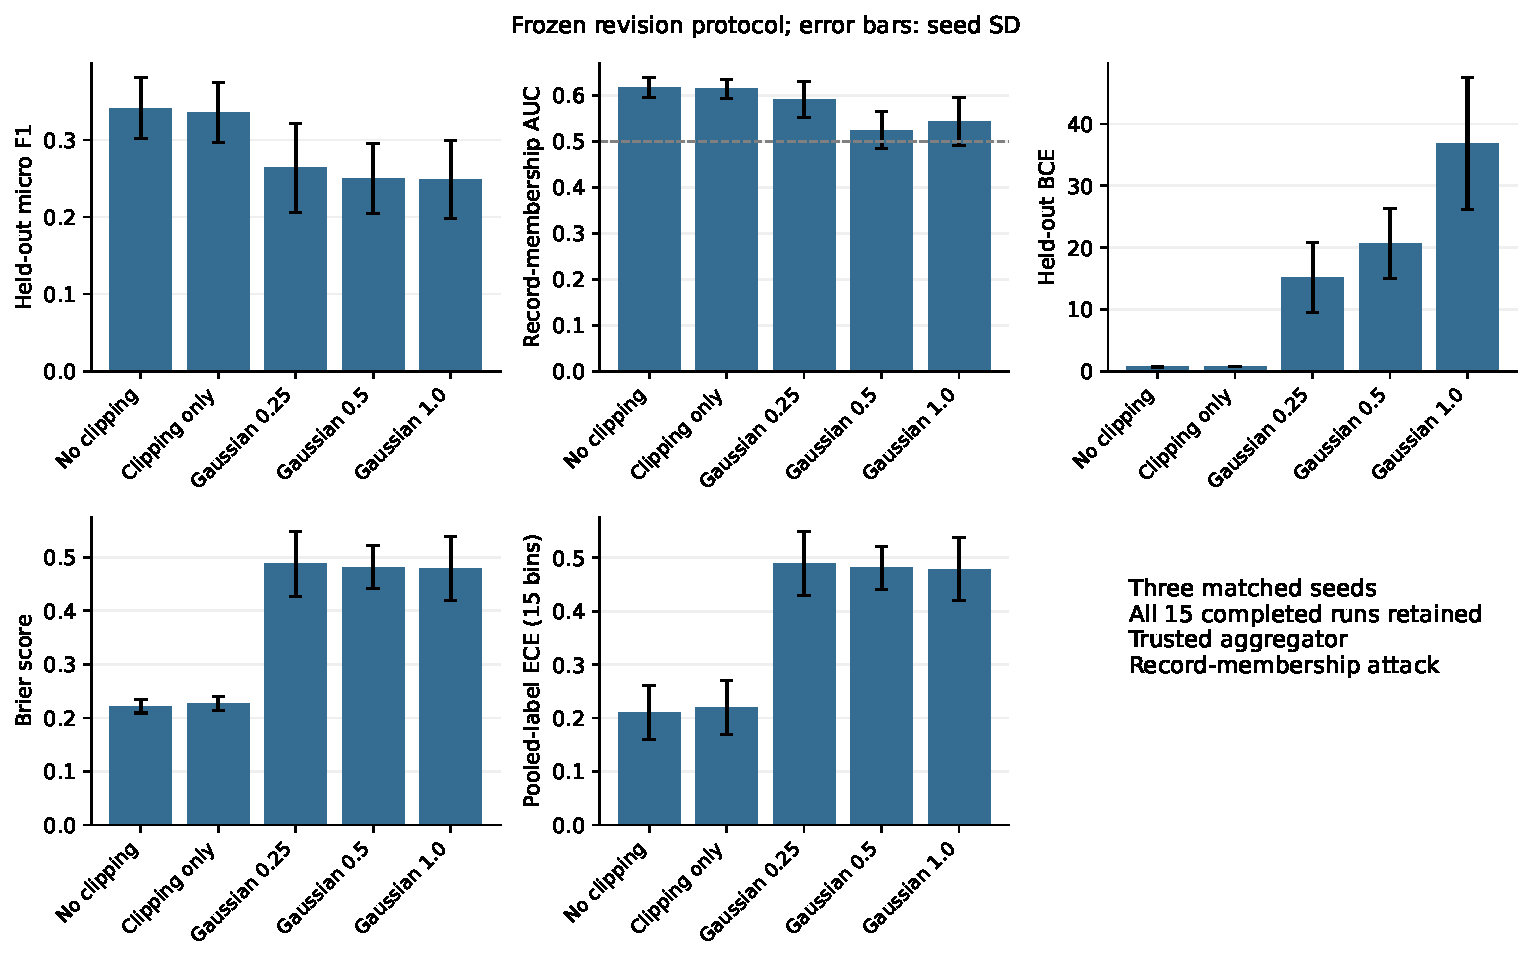
\includegraphics[width=\linewidth]{privacy_utility_attack.pdf}
    \caption{Completed privacy revision over three matched seeds. Bars show means and error bars show one seed standard deviation. The clipping-only control separates clipping from noise. Task performance, record-membership attack AUC, and probability quality are reported as distinct outcomes.}
    \label{fig:privacy-utility-attack}
\end{figure}

\begin{figure}[t]
    \centering
    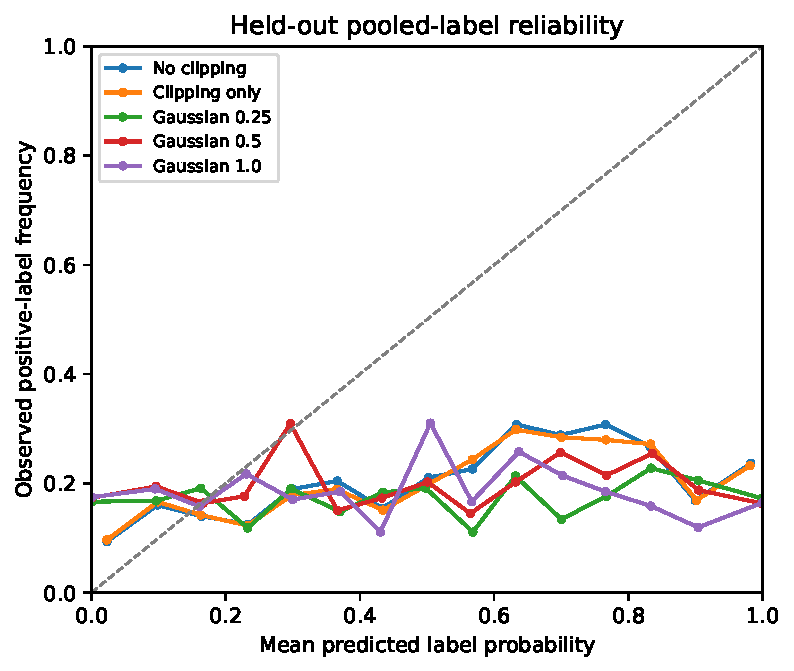
\includegraphics[width=0.68\linewidth]{privacy_reliability.pdf}
    \caption{Held-out English--Polish reliability, pooling binary-label predictions across three seeds within each condition. Each point shows mean probability and observed positive frequency within a fixed probability bin. The dashed diagonal denotes perfect calibration; source data include bin counts.}
    \label{fig:privacy-reliability}
\end{figure}

\FloatBarrier

\IfFileExists{sections/revision_legalbench_results.tex}{%
\subsection{Published-label legal component results}
Eleven of twelve checkpoint conditions have completed the four-task diagnostic; the Mistral 7B reference remains pending model-weight recovery. Table~\ref{tab:revision-legalbench} separates accuracy from class-balanced outcomes. The larger pretrained checkpoint differs in both model family and size; it provides a reference for component difficulty. The released seed and case contrasts include uncertainty, and probability metrics accompany each task.

\begin{table}[t]
\caption{Published-label LegalBench component diagnostics on 492 fixed cases. Entries are percent; adapted rows average five shared checkpoints, pretrained rows evaluate one checkpoint.}
\label{tab:revision-legalbench}
\centering
\small
\resizebox{\linewidth}{!}{%
\begin{tabular}{lrrrr}
\toprule
Task & Checkpoint & Accuracy & Macro F1 & Balanced accuracy \\
\midrule
Overruling & Qwen base & 49.2 & 43.8 & 51.5 \\
Overruling & FedAvg shared & 52.3 & 45.4 & 54.2 \\
Overruling & FLEN shared & 51.8 & 44.9 & 53.5 \\
UCC/common law & Qwen base & 57.4 & 36.5 & 50.0 \\
UCC/common law & FedAvg shared & 57.4 & 36.5 & 50.0 \\
UCC/common law & FLEN shared & 57.4 & 36.5 & 50.0 \\
Citation support & Qwen base & 53.7 & 47.9 & 53.7 \\
Citation support & FedAvg shared & 49.3 & 41.2 & 49.3 \\
Citation support & FLEN shared & 49.1 & 42.4 & 49.1 \\
Personal jurisdiction & Qwen base & 42.0 & 29.6 & 50.0 \\
Personal jurisdiction & FedAvg shared & 54.4 & 46.3 & 56.0 \\
Personal jurisdiction & FLEN shared & 55.2 & 46.4 & 55.2 \\
\bottomrule
\end{tabular}
}
\end{table}


Shared adaptation has task-dependent effects. FedAvg and FLEN reach 52.3\% and 51.8\% on overruling, compared with 49.2\% for the base checkpoint. On citation support, their means fall to 49.3\% and 49.1\% from 53.7\%. All three conditions produce the same UCC/common-law accuracy of 57.4\% with balanced accuracy 50.0\%, revealing a single-class solution. Personal-jurisdiction accuracy increases from 42.0\% to 54.4\% and 55.2\%, while balanced accuracy remains below 56\%. These outcomes identify limited component transfer and motivate expert authority annotation and independently verified citation retrieval.

\begin{figure}[t]
\centering
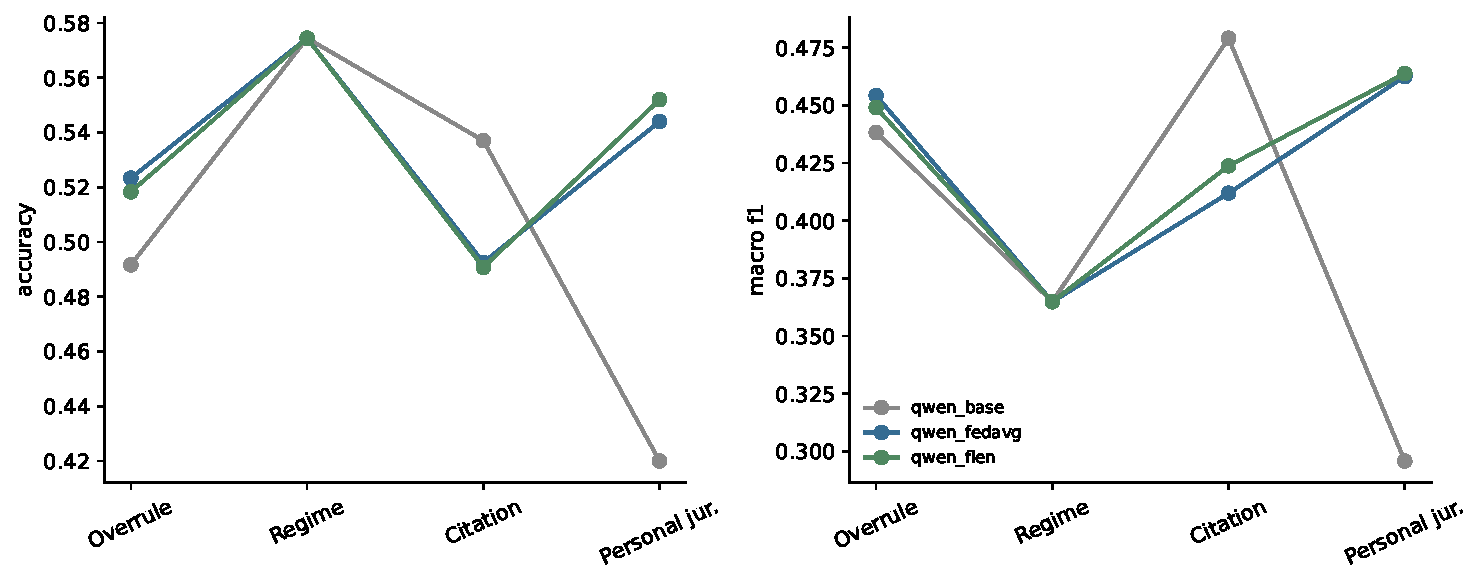
\includegraphics[width=\linewidth]{revision_legalbench.pdf}
\caption{Fixed-case component diagnostics; adapted values average five training seeds. Tasks retain their published label spaces.}
\label{fig:revision-legalbench}
\end{figure}

\FloatBarrier
}{}

\IfFileExists{sections/revision_agents_results.tex}{%
\subsection{Connected shared-adapter reasoning results}
The completed automatic comparison links exported FedAvg and FLEN shared adapters to the same inference protocol as the base checkpoint. Table~\ref{tab:revision-agents} compares role prompting with one-call prediction and four-call self-refinement. These are paired case outcomes for seed-41 checkpoints. Legal soundness, coherence, preference and unsupported-claim rates await completed independent blinded review sheets.

\begin{table}[t]
\caption{Sixty paired reasoning cases per checkpoint. Differences are four-stage minus single-agent accuracy in points; intervals use paired case bootstrap. The four-stage comparator is regenerated deterministically across call-budget packages and counted once.}
\label{tab:revision-agents}
\centering
\small
\resizebox{\linewidth}{!}{%
\begin{tabular}{lrrrrrr}
\toprule
Checkpoint & Single calls & Single (\%) & Four-stage (\%) & Difference & 95\% CI & McNemar $p$ \\
\midrule
base & 1 & 21.7 & 15.0 & $-6.7$ & $[-16.7,3.3]$ & 0.344 \\
base & 4 & 18.3 & 15.0 & $-3.3$ & $[-13.3,6.7]$ & 0.754 \\
federated & 1 & 5.0 & 20.0 & $+15.0$ & $[5.0,25.0]$ & 0.012 \\
federated & 4 & 20.0 & 20.0 & $+0.0$ & $[-5.0,5.0]$ & 1.000 \\
flen & 1 & 1.7 & 25.0 & $+23.3$ & $[13.3,35.0]$ & $<0.001$ \\
flen & 4 & 18.3 & 25.0 & $+6.7$ & $[0.0,15.0]$ & 0.219 \\
\bottomrule
\end{tabular}
}
\end{table}


The one-call FedAvg and FLEN controls parse successfully on only 14 and 10 of 60 cases, respectively. Their large four-stage gains therefore combine task accuracy and output-format compliance. Four-call self-refinement raises successful parsing to 58 and 59 cases. Against that control, four-stage accuracy changes by 0.00 points for FedAvg and 6.67 points for FLEN (95\% paired bootstrap interval $[0.00,15.00]$; exact McNemar $p=0.219$). The base checkpoint decreases by 3.33 points. These call-matched results leave the reasoning advantage uncertain.

\begin{table}[t]
\caption{Output-format diagnostics on 60 cases. S denotes single-agent prediction and D four-stage deliberation. Conditional accuracy (percent) uses only cases parsed in both conditions and is descriptive; primary accuracy retains all cases and counts parsing failures as errors.}
\label{tab:revision-agents-parse}
\centering
\small
\resizebox{\linewidth}{!}{%
\begin{tabular}{lrrrrrr}
\toprule
Checkpoint & Single calls & Parsed S & Parsed D & Both & Cond. acc. S & Cond. acc. D \\
\midrule
base & 1 & 58 & 55 & 53 & 18.9 & 17.0 \\
base & 4 & 58 & 55 & 54 & 16.7 & 16.7 \\
federated & 1 & 14 & 60 & 14 & 21.4 & 14.3 \\
federated & 4 & 58 & 60 & 58 & 20.7 & 19.0 \\
flen & 1 & 10 & 59 & 10 & 10.0 & 10.0 \\
flen & 4 & 59 & 59 & 58 & 19.0 & 24.1 \\
\bottomrule
\end{tabular}
}
\end{table}


\begin{table}[t]
\caption{Mean analysis cost per case with four calls in both conditions. The common presentation step is excluded; call matching does not match token consumption.}
\label{tab:revision-agents-cost}
\centering
\small
\resizebox{\linewidth}{!}{%
\begin{tabular}{lrrrr}
\toprule
Checkpoint & Protocol & Prompt tokens & Generated tokens & Seconds \\
\midrule
base & Self-refinement & 1942.7 & 96.7 & 1.68 \\
base & Four-stage & 2711.1 & 447.5 & 7.69 \\
federated & Self-refinement & 2074.6 & 251.0 & 5.70 \\
federated & Four-stage & 2635.5 & 375.6 & 8.51 \\
flen & Self-refinement & 2081.5 & 256.4 & 6.43 \\
flen & Four-stage & 2601.0 & 360.2 & 8.93 \\
\bottomrule
\end{tabular}
}
\end{table}


For the FLEN checkpoint, four-stage analysis consumes 360.3 generated tokens and 8.93 seconds per case, compared with 256.4 tokens and 6.43 seconds for self-refinement. The extra deliberation therefore increases generated tokens by about 41\% and observed elapsed time by about 39\%.

\begin{figure}[t]
\centering
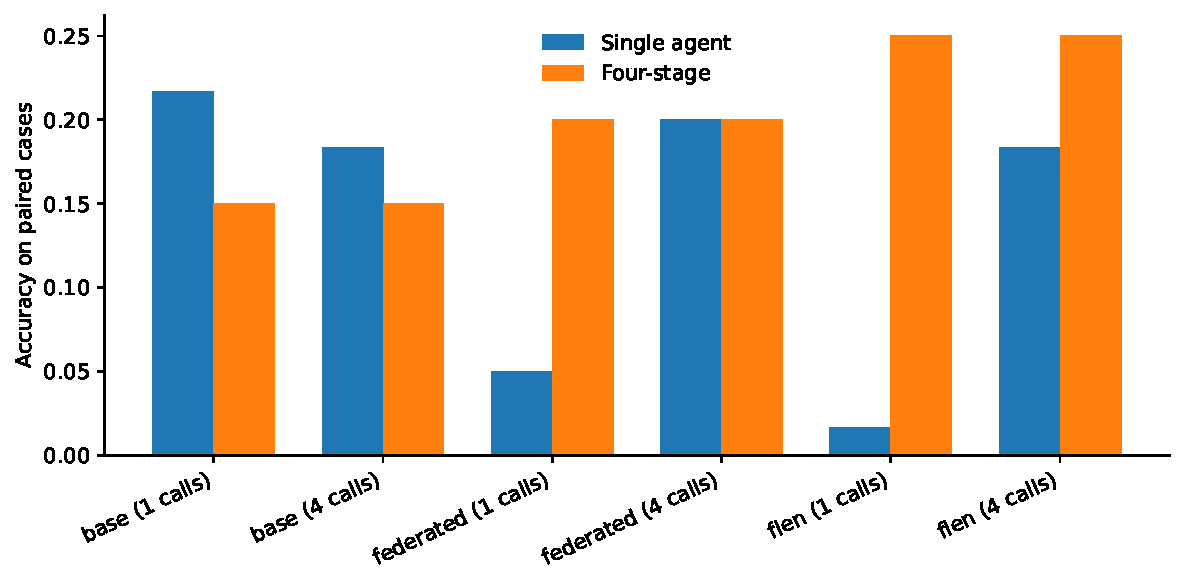
\includegraphics[width=\linewidth]{revision_agents.pdf}
\caption{Automatic paired accuracy with base, FedAvg shared and FLEN shared checkpoints; call budgets label the single-agent controls.}
\label{fig:revision-agents}
\end{figure}

}{%
\subsection{Legacy paired multi-agent diagnostic and blinded review package}

The legacy inference study compares a single legal analyst with a typed four-stage workflow comprising primary analysis, adversarial challenge, evidence verification, and final judgement. It loads the base model; the experiment evaluates role prompting rather than the effect of federated adaptation. Both conditions use deterministic decoding and the same presentation step, which renders a selected holding and two-sentence explanation before per-case A/B randomization. The 60-case package contains the anonymous review sheet, a separately stored method key, raw predictions, a concise holistic rubric, and an adjudication protocol for two legally trained reviewers.

\begin{table}[t]
\caption{Paired automatic CaseHOLD diagnostic on 60 cases. Exclusive correct counts cases solved by one condition and missed by the other.}
\label{tab:multi-agent-automatic}
\centering
\begin{tabular}{lccc}
\toprule
Condition & Accuracy (\%) & Parse rate (\%) & Exclusive correct \\
\midrule
Single agent & 18.33 & 96.67 & 2 \\
Typed four-stage deliberation & 21.67 & 95.00 & 4 \\
\bottomrule
\end{tabular}
\end{table}


Table~\ref{tab:multi-agent-automatic} reports the completed automatic diagnostic. Typed deliberation improves accuracy from 18.33\% to 21.67\%, a paired difference of $+3.33$ points. The 95\% paired bootstrap interval is $[-5.00,11.67]$ points, and the exact McNemar test gives $p=0.6875$. The direction is positive but the interval includes zero. Human preference, legal soundness, reasoning coherence, and unsupported-claim rates will be computed after two independent review sheets are frozen and disagreements are adjudicated.

\FloatBarrier

}
\section{Discussion}

\paragraph{Frozen revision protocol.}
The revised CaseHOLD protocol specifies independent additive LoRA branches, five matched seeds, twenty rounds, and 1,200 training records. It compares gating at fixed eight-shared/two-private and ten-shared/two-private step schedules, with the same gate records excluded from both phases. FedAvg, FedProx, and Ditto provide shared and personalized baselines. A fixed 1,000-record test sample is evaluated after the final training round, with aggregate and worst-client accuracy, compute, drift, and logical communication recorded. The language experiment reserves aggregation probes from the training split separately from threshold-validation data. The completed privacy revision includes a clipping-only control, a 0.25 noise condition, Brier score and calibration error; its record non-members come from the test split. The agent protocol crosses base and federated-adapter models with single-agent and four-stage prompting and includes a four-call self-refinement control. Revision results are distinguished from the legacy screening. Expert annotation uses official authority sources with source-family separation; completed human labels and independent reasoning reviews are required to report their corresponding outcomes.

The central design principle is that legal heterogeneity includes sampling variation, task mismatch, model error, and legitimate authority-scoped disagreement. FLEN separates these sources through a comparability gate, target-conditioned cohorts, jurisdiction-local residuals, and a diversity floor. This design protects a legally valid minority jurisdiction from unconditional conflict downweighting. Expert-labelled probes provide the construct-validity test for the resulting categories.

The evidence establishes reproducible target-conditioned Flower/PEFT execution, active conflict weighting, and adverse personalization in the legacy factor-residual implementation. The revised dual-branch experiment tests gate attribution at fixed training budgets. MultiEURLEX shows that source-language adaptation improves over an unadapted backbone, while target-language local supervision remains substantially stronger. Proxy-FLEN changes weights consistently but does not outperform FedAvg within the three-seed interval. The measured scope is proxy non-IID optimization and multilingual EU-law transfer under a shared authority.

The completed privacy revision identifies a three-client regime with sharply increased probability loss, Brier score, and calibration error. Record-membership AUC is closer to 0.5 under the tested noise conditions, with paired intervals that include zero and a non-monotonic noise response. The paired agent diagnostic shows a positive but uncertain automatic accuracy difference. Expert conflict labels, authentic jurisdiction partitions, and the two-reviewer blinded assessment determine whether the mechanism extends from proxy optimization to legally meaningful cross-jurisdiction transfer.

\section{Ethics, Governance, and Intended Use}

FLEN supports legal information processing and decision support under accountable human authority. Institutional use requires access to supporting authorities and uncertainty records, an appeal or override path, and documented responsibility for model and data governance. The system abstains when a rule lacks support or a jurisdictional conflict remains unresolved.

The measured pilot uses public benchmarks. Institutional studies document legal basis, data licences, retention, access control, cross-border restrictions, and the treatment of sealed or personally identifiable information. Reasoning summaries and audit trails may themselves be sensitive and require minimization, purpose limitation, and deletion policies.

Fairness evaluation includes minority jurisdictions and affected groups alongside aggregate utility. Qualified legal experts from the represented jurisdictions create or audit the authority mapping and conflict benchmark, with disagreement and uncertainty retained in the annotations. Privacy and policy auditors support traceability; legal oversight, independent security review, and empirical bias assessment remain required governance controls.

\section{Conclusion}

This paper specifies FLEN, a data-local federated framework that separates transfer eligibility from raw client disagreement. Conflict diagnostics operate on comparable probes, shared adapters are target-conditioned, jurisdiction-local residuals use train-internal selection, and typed deliberation supports verification before synthesis. Legacy CaseHOLD experiments show active conflict weighting and adverse personalization; the revised implementation tests independent branches and matched-budget gating. MultiEURLEX experiments show an adaptation gain over the unadapted reference and a substantial gap to target-supervised local adaptation, with an uncertain proxy-FLEN effect over FedAvg. The client-update privacy screen quantifies changes in record-membership attack AUC and probability loss, while the 60-case agent diagnostic remains statistically inconclusive. Expert-adjudicated conflict labels, authentic jurisdiction partitions, and completed blinded legal review provide the next tests of legal transfer and reasoning quality.

\section*{Data and code availability}
The manuscript source, implementation, experiment configurations, analysis scripts, and published result summaries are available at \url{https://github.com/Robert-solo/federated_legal.git}. The repository documents the software environment, random seeds, execution commands, and the correspondence between reported tables, figures, and source runs. The latest Elsevier CAS manuscript is the maintained paper version. Benchmark datasets are obtained from their original providers under their respective licences. Expert annotations and blinded-review outcomes are released with their provenance after human review is completed.




\bibliography{custom}

\end{document}
